\documentclass[a4paper, 12pt, oneside, openany, final, pdftex]{book}\usepackage[]{graphicx}\usepackage[]{color}
%% maxwidth is the original width if it is less than linewidth
%% otherwise use linewidth (to make sure the graphics do not exceed the margin)
\makeatletter
\def\maxwidth{ %
  \ifdim\Gin@nat@width>\linewidth
    \linewidth
  \else
    \Gin@nat@width
  \fi
}
\makeatother

\definecolor{fgcolor}{rgb}{0.345, 0.345, 0.345}
\newcommand{\hlnum}[1]{\textcolor[rgb]{0.686,0.059,0.569}{#1}}%
\newcommand{\hlstr}[1]{\textcolor[rgb]{0.192,0.494,0.8}{#1}}%
\newcommand{\hlcom}[1]{\textcolor[rgb]{0.678,0.584,0.686}{\textit{#1}}}%
\newcommand{\hlopt}[1]{\textcolor[rgb]{0,0,0}{#1}}%
\newcommand{\hlstd}[1]{\textcolor[rgb]{0.345,0.345,0.345}{#1}}%
\newcommand{\hlkwa}[1]{\textcolor[rgb]{0.161,0.373,0.58}{\textbf{#1}}}%
\newcommand{\hlkwb}[1]{\textcolor[rgb]{0.69,0.353,0.396}{#1}}%
\newcommand{\hlkwc}[1]{\textcolor[rgb]{0.333,0.667,0.333}{#1}}%
\newcommand{\hlkwd}[1]{\textcolor[rgb]{0.737,0.353,0.396}{\textbf{#1}}}%
\let\hlipl\hlkwb

\usepackage{framed}
\makeatletter
\newenvironment{kframe}{%
 \def\at@end@of@kframe{}%
 \ifinner\ifhmode%
  \def\at@end@of@kframe{\end{minipage}}%
  \begin{minipage}{\columnwidth}%
 \fi\fi%
 \def\FrameCommand##1{\hskip\@totalleftmargin \hskip-\fboxsep
 \colorbox{shadecolor}{##1}\hskip-\fboxsep
     % There is no \\@totalrightmargin, so:
     \hskip-\linewidth \hskip-\@totalleftmargin \hskip\columnwidth}%
 \MakeFramed {\advance\hsize-\width
   \@totalleftmargin\z@ \linewidth\hsize
   \@setminipage}}%
 {\par\unskip\endMakeFramed%
 \at@end@of@kframe}
\makeatother

\definecolor{shadecolor}{rgb}{.97, .97, .97}
\definecolor{messagecolor}{rgb}{0, 0, 0}
\definecolor{warningcolor}{rgb}{1, 0, 1}
\definecolor{errorcolor}{rgb}{1, 0, 0}
\newenvironment{knitrout}{}{} % an empty environment to be redefined in TeX

\usepackage{alltt}

  \newcommand{\documentVersion}{1.2}
\newcommand{\FacultyNameCro}{Faklultet Organizacije i Informatike}
\newcommand{\FacultyNameEng}{Faculty of Organization and Informatics}
\newcommand{\AuthorNameSurname}{Matija Novak}
\newcommand{\ThesisTitleEng}{Some very very very very very very looooooong title}
\newcommand{\ThesisTitleCro}{Neki jako jako jako jako jako jako veliiiiiki naslov}
\newcommand{\ThesisKeywords}{key1, key2, ke3}

  
  % PAKETI

% geometrija stranice
% margine postavljene kao sto i pise u obrascu DR.SC.08
\usepackage[margin=25mm,centering]{geometry} 

% prihvaca tex kod kao UTF-8 omogućavajući
% pisanje znakova s dijakriticima unutar datoteke
% npr. možemo pisati 'č' umjesto č
% PAZITI DA SU DATOTEKE STVARNO SPREMLJENE KAO UTF-8
% nije korisno ako se namjerava koristiti 'latexdiff'
\usepackage[utf8]{inputenc}

% omogućiti ispisivanje naših znakova u dokumentu 
\usepackage[T1]{fontenc}

% koristi novu verziju fonta (Latin Modern)
%\usepackage{lmodern}

% Palatino font (blizu Arial-a)
%\usepackage[sc]{mathpazo}
\usepackage{uarial}

% Times New Roman
\usepackage{mathptmx}
% ili
%\usepackage{txfonts}

% koristan paket kad stvaranja pdf-a
\usepackage[activate={true,nocompatibility},
	final,
	tracking=true,
	kerning=true,
	spacing=true,
	factor=1100,
	stretch=10,
	shrink=10]{microtype}
\microtypecontext{spacing=nonfrench}
%\usepackage{microtype}

% babel !
\usepackage[croatian, english]{babel}
\usepackage{csquotes}
%\usepackage{hyphenat}
 

% captioni ce biti centrirani te će im ime biti podebljano. 
\usepackage[center,labelfont=bf]{caption}

%center command without adding spaces before and after
\newenvironment{nscenter}
 {\parskip=0pt\par\nopagebreak\centering}
 {\par\noindent\ignorespacesafterend}

% koristan paket za pisanje url-ova u tekstu
\usepackage{url}

% paketi za oblikovanje tablica
\usepackage{booktabs}
\usepackage{multirow}
\usepackage{array}
\newcolumntype{t}{>{\ttfamily}c}

% paketi za oblikovanje lista
\usepackage[ampersand]{easylist}
\usepackage{enumitem}

% boje, bojice, jeee :D
\usepackage{color}
\usepackage[table]{xcolor}
\definecolor{dark-red}{rgb}{0.4,0.15,0.15}
\definecolor{dark-blue}{rgb}{0.15,0.15,0.4}
\definecolor{medium-blue}{rgb}{0,0,0.5}
\definecolor{black}{rgb}{0,0,0}
\definecolor{fgcolor}{rgb}{0.345, 0.345, 0.345} %needed for R


% dodatni simboli
\usepackage{pifont}

% glossaries
\usepackage{supertabular}
\usepackage[nomain,acronym,nonumberlist,style=list,translate=false]{glossaries}


% prilagođavanje oblika naslova poglavalja (chapter),
% potpoglavlja (section) i odjeljka (subsection)
\usepackage{titlesec}
	\titleformat{\chapter}[display]
	{\normalfont \centering}%format
	{\fontsize{10}{12} \selectfont \uppercase{chapter} \thechapter}%label
	{0.5ex}%sep
	{\fontsize{18}{20} \selectfont \bfseries \MakeUppercase} %before-title-code
	[\vspace{-0.5ex} \rule{\textwidth}{0.3pt}] %after-title-code
  \titlespacing*{\chapter}{0pt}{0pt}{6pt}	

	\titleformat{\section}
	{\normalfont \fontsize{16}{18} \selectfont \bfseries}%format
	{\thesection}%label
	{5pt}%sep
	{}%before-title-code
	\titlespacing*{\section}{0pt}{18pt}{6pt}
	
	\titleformat{\subsection}
	{\normalfont \fontsize{14}{16} \selectfont \bfseries}%format
	{\thesubsection}%label
	{5pt}%sep
	{}%before-title-code
	\titlespacing*{\subsection}{0pt}{12pt}{6pt}

% crtanje !
\usepackage{tikz}

% verbatim env.
\usepackage{moreverb}

% multi tables/figures
\usepackage{subcaption}
\usepackage{float}
\usepackage{makecell}
\usepackage{longtable}
\usepackage{colortbl}
\usepackage{tabu}
\usepackage{threeparttable}
\usepackage{threeparttablex}
\usepackage[normalem]{ulem}
\usepackage{wrapfig}

%source code
\usepackage{listings}
\lstset{
  language=Java,
  basicstyle=\small,
  breaklines=true
  }

% uklucivanje slika
\usepackage{graphicx}
\usepackage{epstopdf}

% matematika
\usepackage{amssymb ,amsmath, amsthm, amsfonts}
\usepackage{enumitem}
\allowdisplaybreaks[1]
\usepackage{bbm}
\usepackage{xfrac} % xfrac je koristan paket za umetanje razlomaka unutar teksta

% headeri i footeri
\usepackage{fancyhdr}

% hack za fancyhdr i problem s headerheight-om
% http://nw360.blogspot.com/2006/11/latex-headheight-is-too-small.html
\setlength{\headheight}{15pt}

% paketi za pisanje algoritama
%\usepackage{algorithmic}
\usepackage[croatian,	linesnumbered, onelanguage]{algorithm2e}

% EUROPSKI NACIN RAZDVAJANJA ODLOMAKA
%\setlength{\parskip}{1ex plus 0.5ex minus 0.2ex}
%\setlength{\parindent}{0pt}

% indentacija na prvom paragrafu u poglavlju
\usepackage{indentfirst}

% macroi, naredbe i slicno
\usepackage{xparse}


% podesi prored na 1.5
\usepackage[onehalfspacing]{setspace}

% dodaje random tekst
\usepackage{lipsum}

% paketi za referenciranje
%\usepackage{varioref}
%\usepackage{cleveref}

% BIBLIOGRAFIJA

% koristiti biber s dodatkom za hrvatski jezik
% kod kompajliranja dokumenta!!!

% paket za upravljanje bibliografijom
%\usepackage[style=authoryear,citestyle=authoryear,doi=false,isbn=false,dashed=false,
%  maxcitenames=2,maxbibnames=100]{biblatex}
\usepackage[backend=bibtex,
  doi=true,
	isbn=true,
	url=false,
	maxbibnames=100,
	defernumbers=true,
	sorting=nyt,
	style=ieee,
	dashed=false,
	citestyle=numeric-comp]{biblatex}
\AtEveryBibitem{\clearfield{note}}

% pogledati 
% https://tex.stackexchange.com/questions/111363/exclude-fullcite-citation-from-bibliography
% za objasnjenje sljedece tri linije
% korisno ako zelimo printati s \fullcite bibligrafiju u zivotopisu
% a taj se clanak ne pojavljuje citiran u ostatku disertacije
\DeclareBibliographyCategory{fullcited}
\newcommand{\mybibexclude}[1]{\addtocategory{fullcited}{#1}}

% Izgled stranica (header, footer, ...)

\fancypagestyle{plain}{
	\fancyhf{} 
	\renewcommand{\headrulewidth}{0pt}
	\renewcommand{\footrulewidth}{0pt}
	\fancyfoot[R]{\thepage} 

	% sljedeća linija dodaje u footer informaciju o trenutnoj verziji dokumenta
	% potrebno ju je zakomentirati kod finalnog ispisa
	\fancyfoot[L]{\nouppercase{\footnotesize \today : version \documentVersion}} 
}

\pagestyle{fancy}{
	\fancyhf{} 
	%\renewcommand{\headrulewidth}{0pt}
	%\renewcommand{\footrulewidth}{0pt}
	\rhead{\nouppercase{\footnotesize \leftmark}}
	\fancyfoot[R]{\thepage} 

	% sljedeća linija dodaje u footer informaciju o trenutnoj verziji dokumenta
	% potrebno ju je zakomentirati kod finalnog ispisa
	\fancyfoot[L]{\nouppercase{\footnotesize \today : version \documentVersion}} 
}
\pagestyle{fancy}

% potrebno za dodavanje naslovnice u finalni dokument
\usepackage{pdfpages}

% postavi velicinu razmaka nakon znaka '.' (tocka) 
% uvijek na istu vrijednost. Inace ce razmak biti
% veci na kraju recenice nego kod skracenica npr.
%\frenchspacing

% korisno za provjeravanje dokumenta u finalnoj fazi
%\usepackage{refcheck}
%\usepackage{showkeys}

% korisno za mjenjanje jedne stranice u landscape mode
\usepackage{pdflscape}

%appendix da se dobro prikazuje u popisu i u naslovu kod samog appendixa umjesto Chapter
\usepackage[titletoc]{appendix}

% paket za stvaranje poveznica u elektronskom
% dokumentu. Koristan kod objavljivanja elektronskog
% oblika dokumenta
\usepackage[final]{hyperref}

\PassOptionsToPackage{unicode}{hyperref}
\PassOptionsToPackage{naturalnames}{hyperref}

\hypersetup{
	unicode=true,       % non-Latin characters in Acrobat’s bookmarks
	pdfauthor={\AuthorNameSurname},
	pdftitle={\ThesisTitleEng},
	pdfsubject={},
	pdfkeywords={\ThesisKeywords},
	colorlinks=true,    % false: boxed links; true: colored links
	linkcolor={black},  % color of internal links (change box color with linkbordercolor)
	citecolor={black},  % color of links to bibliography
	urlcolor={black}    % color of external links
}

% za review
\usepackage{soul} % precrtaj korisit \st{}
\newcommand{\remove}[1]{\textcolor{red}{}}
\newcommand{\add}[1]{\textcolor{blue}{#1}}
  
  %%%%%%%%%%%%%%%%%%%%%%%%%%%%%%%%%%%%%%%%%%%%%%%%%%%%%%%%
% ENVIRONMENTI
%%%%%%%%%%%%%%%%%%%%%%%%%%%%%%%%%%%%%%%%%%%%%%%%%%%%%%%%
%
\NewDocumentEnvironment{primjer_}{o}
{
	\refstepcounter{tm}
	\IfNoValueTF {#1}
	{ 
		\noindent
		{\textbf{Primjer \thechapter.\arabic{tm}}}}
	{ 
		\noindent
		{\textbf{Primjer \thechapter.\arabic{tm}} (#1)}}
}
{ \hspace*{\stretch{1}}\rule{1ex}{1ex} }

\NewDocumentEnvironment{output_}{o}
{
	\refstepcounter{tm}
	\IfNoValueTF {#1}
	{ 
		\noindent
		{\textbf{Ouptut \thechapter.\arabic{tm}}}}
	{ 
		\noindent
		{\textbf{Ouptut \thechapter.\arabic{tm}} (#1)}}
}
{ \hspace*{\stretch{1}}\rule{1ex}{1ex} }

\NewDocumentEnvironment{napomena_}{o}
{
	\refstepcounter{tm}
	\IfNoValueTF {#1}
	{ 
		\noindent
		{\textbf{Napomena \thechapter.\arabic{tm}}}}
	{ 
		\noindent
		{\textbf{Napomena \thechapter.\arabic{tm} } (#1)}}
}
{ \hspace*{\stretch{1}}\rule{1ex}{1ex} }

  
  %%%%%%%%%%%%%%%%%%%%%%%%%%%%%%%%%%%%%%%%%%%%%%%%%%%%%%%%%%%%%%%%%%%%%%%%%%%%%%%%
% KORISNE KRATICE (teoremi, definicije, ...)
%%%%%%%%%%%%%%%%%%%%%%%%%%%%%%%%%%%%%%%%%%%%%%%%%%%%%%%%%%%%%%%%%%%%%%%%%%%%%%%%

\newtheoremstyle{stil}{}{}{}{}{\bfseries}{}{ }{}
\theoremstyle{stil}
\newtheorem{tm}{Teorem}[chapter]
\newtheorem{defn}[tm]{Definicija}
\newtheorem{pro}[tm]{Propozicija}
\newtheorem{prop}[tm]{Propozicija}
\newtheorem{lem}[tm]{Lema}
\newtheorem{kor}[tm]{Korolar}

%%%%%%%%%%%%%%%%%%%%%%%%%%%%%%%%%%%%%%%%%%%%%%%%%%%%%%%%
% KORISNE KRATICE (komande)
%%%%%%%%%%%%%%%%%%%%%%%%%%%%%%%%%%%%%%%%%%%%%%%%%%%%%%%%

% za dodavanje todo dijelova
\newcommand{\todo}[1]{\textcolor{red}{#1}}
%za citirane dijelove i dijelove pod navodnicima
\newcommand{\udquote}[1]{``\textit{#1}''}
\newcommand{\udquotehr}[1]{„#1”}

% koristimo kod prvog pojavljivanja pojma
\newcommand{\be}[1]{\textbf{\em{#1}}}

% konvergencija
\newcommand{\konv}[2]{#1 \rightarrow #2}

% konvergencija gotovo sigurno
\newcommand{\konvgs}[2]{#1 \xrightarrow{g.s.} #2}
\newcommand{\nkonvgs}[2]{#1 \not \xrightarrow{g.s} #2}
% konvergencija po vjerojatnosti
\newcommand{\konvpv}[2]{#1 \xrightarrow{P} #2}
\newcommand{\nkonvpv}[2]{#1 \not \xrightarrow{P} #2}
% konvergencija po distribuciji
\newcommand{\konvpd}[2]{#1 \xrightarrow{D} #2}
\newcommand{\nkonvpd}[2]{#1 \not \xrightarrow{D} #2}
% konvergencija u srednjem
\newcommand{\konvusr}[3]{#1 \xrightarrow{L^{#3}} #2}
\newcommand{\nkonvusr}[3]{#1 \not \xrightarrow{L^{#3}} #2}

% skalar
\newcommand{\ts}[1]{\lowercase{#1}}
% vektor
\newcommand{\tv}[1]{\mathbf{\lowercase{#1}}}
% matrica 
\newcommand{\tmatrix}[1]{\uppercase{#1}}
% tenzor
\newcommand{\ttenzor}[1]{\mathbf{\uppercase{#1}}}
% slucajna varijabla
\newcommand{\tsvar}[1]{\uppercase{#1}}
% slucajan vektor
\newcommand{\tsvek}[1]{\uppercase{\textbf{#1}}}

% niz znakova od interesa
\newcommand{\nz}[1]{{\sc #1}}
% specijalno za DNA kao hack da ih prvo spusti
% jer sam ih pisao velikim slovima
\newcommand{\nzdna}[1]{{\sc{\lowercase{#1}}}}
% specijalno za slicnost stringova
% jer se small caps ne prikazuje najbolje u math modu
\newcommand{\nzk}[1]{{\textit{#1}}}

% povlaka nad slovom u math modu
\newcommand{\ol}[1]{\widetilde{#1}}

% dupla povlaka nad slovom
% u math modu
\newcommand{\dol}[1]{\ol{\ol{#1}}}

% povlaka nad slovom u textmodu
\newcommand{\tol}[1]{\~{#1}}

%%%%%%%
% vjerojatnosni simboli
\newcommand{\vP}{\mathrm{P}}
\newcommand{\vE}[1]{\mathrm{E}\left(#1\right)}
\newcommand{\vVar}[1]{\mathrm{Var}\left(#1\right)}
\newcommand{\vCov}[1]{\mathrm{Cov}\left(#1\right)}


%%%%%%%
% matematicki skupovi
\newcommand{\setN}{\mathbb{N}}
\newcommand{\setZ}{\mathbb{Z}}
\newcommand{\setQ}{\mathbb{Q}}
\newcommand{\setR}{\mathbb{R}}
\newcommand{\setC}{\mathbb{C}}
\newcommand\scalemath[2]{\scalebox{#1}{\mbox{\ensuremath{\displaystyle #2}}}}


%%%%%%%
% neke funkcije/operatori
\DeclareMathOperator{\tg}{tg}
\DeclareMathOperator{\ctg}{ctg}
\DeclareMathOperator{\arctg}{arctg}
\DeclareMathOperator{\arcctg}{arcctg}
\DeclareMathOperator{\sh}{sh}
\DeclareMathOperator{\tgh}{th}
\DeclareMathOperator{\cth}{cth}
\DeclareMathOperator{\Ker}{Ker}
\DeclareMathOperator{\slika}{Im}
\DeclareMathOperator{\rang}{rang}
\DeclareMathOperator{\vek}{vec}
\DeclareMathOperator{\Span}{span}

%%%%%%%
% ostalo
\newcommand{\mbold}[1]{\mathbf{#1}}
\newcommand{\diag}{\mathop{\mathrm{diag}}}


  
  \newacronym{PPT}{PPT}{PreProcessing Technique}
\newacronym{CCR}{CCR}{Common Code Remove}
\newacronym{MLM}{MLM}{Common Code Remove}
\newacronym{SOCO}{SOCO}{Common Code Remove}

\newglossaryentry{rulebasedapproach}
{
  name=pristup korištenjem pravila asdf asdf asdf asdfas asdf asdgf aasdf,
  description={rule-based approach fdsag asdfg sdafg sdfg sdfg sdfg sdfgsdfg sdfg sdfg sdfg sdfgsdfgs sdfg sfg sdfg sdfgsdfg}
}

\newglossaryentry{Linux}
{
  name=Linux,
  description={is a generic term referring to the family of Unix-like
               computer operating systems that use the Linux kernel},
  plural=Linuces
}

\newacronym[longplural={Frames per Second}]{fpsLabel}{FPS}{Frame per Second} \makeglossaries
  
  \addbibresource{bibAndGlossary/myArticles.bib}
  \addbibresource{bibAndGlossary/reviewArticles.bib}
  \addbibresource{bibAndGlossary/reviewManualyAdded.bib}
  \addbibresource{bibAndGlossary/otherArticlesPhd.bib}
\IfFileExists{upquote.sty}{\usepackage{upquote}}{}
\begin{document}
  \selectlanguage{english} %croatian
  \restoregeometry
  
  \pdfbookmark{Title page}{titlePage}
  
\includepdf[pages=-]{./title-pages/allTitlePages.pdf}

  \frontmatter
    \pagenumbering{Roman}
    
    \pdfbookmark[1]{Acknowledgments}{acknowledgments}
\chapter*{Acknowledgments}
\markboth{Acknowledgments}{Acknowledgments}

\lipsum[1-4]

\ldots
    \cleardoublepage
\pdfbookmark[1]{Abstract}{abstract}
\chapter*{Abstract}
\markboth{Abstract}{Abstract}

\lipsum[1-4]

\ldots
    \cleardoublepage
\pdfbookmark[1]{Sažetak}{sazetak}
\chapter*{Prošireni sažetak}
\markboth{Prošireni sažetak}{Prošireni sažetak}

\lipsum[1-4]

\ldots

Some \udquotehr{asdf} \cite{hebb1985social} 

\lipsum[1-4]

\ldots
    \cleardoublepage
\pdfbookmark[1]{Keywords}{keywords}
\chapter*{Keywords}
\markboth{Keywords}{Keywords}

\begin{center}
	\textit{ 
	\ThesisKeywords
}
\end{center}


    
    \cleardoublepage
    \pdfbookmark{Contents}{tableOfContents}
    \fontsize{10}{11} \selectfont \tableofcontents
    \normalsize \selectfont
    
    \cleardoublepage
    \pdfbookmark[1]{List of figures}{figureList}
    \listoffigures
    
    \cleardoublepage
    \pdfbookmark[1]{List of tables}{tableList}
    \listoftables
    
    % za pojasnjenje naredbi \cleardoublepage i \phantomsection
    % pogledati:
    % https://tex.stackexchange.com/questions/57427/how-to-add-printindex-to-tableofcontents
    % https://tex.stackexchange.com/questions/9191/when-do-i-need-invoke-clearpage-manually
    % https://tex.stackexchange.com/questions/44088/when-do-i-need-to-invoke-phantomsection
    \cleardoublepage
    \pdfbookmark[1]{Glossary}{glossary}
    \printglossary[title=Glossary,toctitle=Terms and abbreviations]
  
  \mainmatter

    

\chapter{Introduction}\label{ch:introducion}
\lipsum[1-4]

\ldots

Cites examples \cite{ryan1991motivational, hebb1985social, Saxon2000} some footnote\footnote{footnote text} level.  

The overall goal of this research is to :
\begin{itemize}
  \item[G1]: \textit{Goal 1}
  \item[G2]: \textit{Goal 2.}
\end{itemize}
From the goals the following hypotheses emerge:
\begin{itemize}
  \item[H1]: \textit{Hip 1}
  \item[H2]: \textit{Hip 2}
\end{itemize}
Since G2 is partially fulfilled by H2 the rest is covered by the following research question:
\begin{itemize}
  \item[Q1]: \textit{Queston}
\end{itemize}

The rest of the thesis is structured as follows. In Chapter \ref{ch:relatedwork}, related work is described including short sections describing ... Chapter \ref{ch:methodology} ... Conclusion \ref{ch:conclusion} concludes. \cite{ottenstein1976, leach1995}
 
Glossary \gls{PPT} and plural \glspl{PPT} and \gls{CCR}


\chapter{Related work}\label{ch:relatedwork}
\lipsum[1-4]

\ldots

\chapter{Methodology}\label{ch:methodology}

\lipsum[1-4]

\ldots 

 \begin{figure}[tb]
 	\centering
\begin{knitrout}
\definecolor{shadecolor}{rgb}{0.969, 0.969, 0.969}\color{fgcolor}
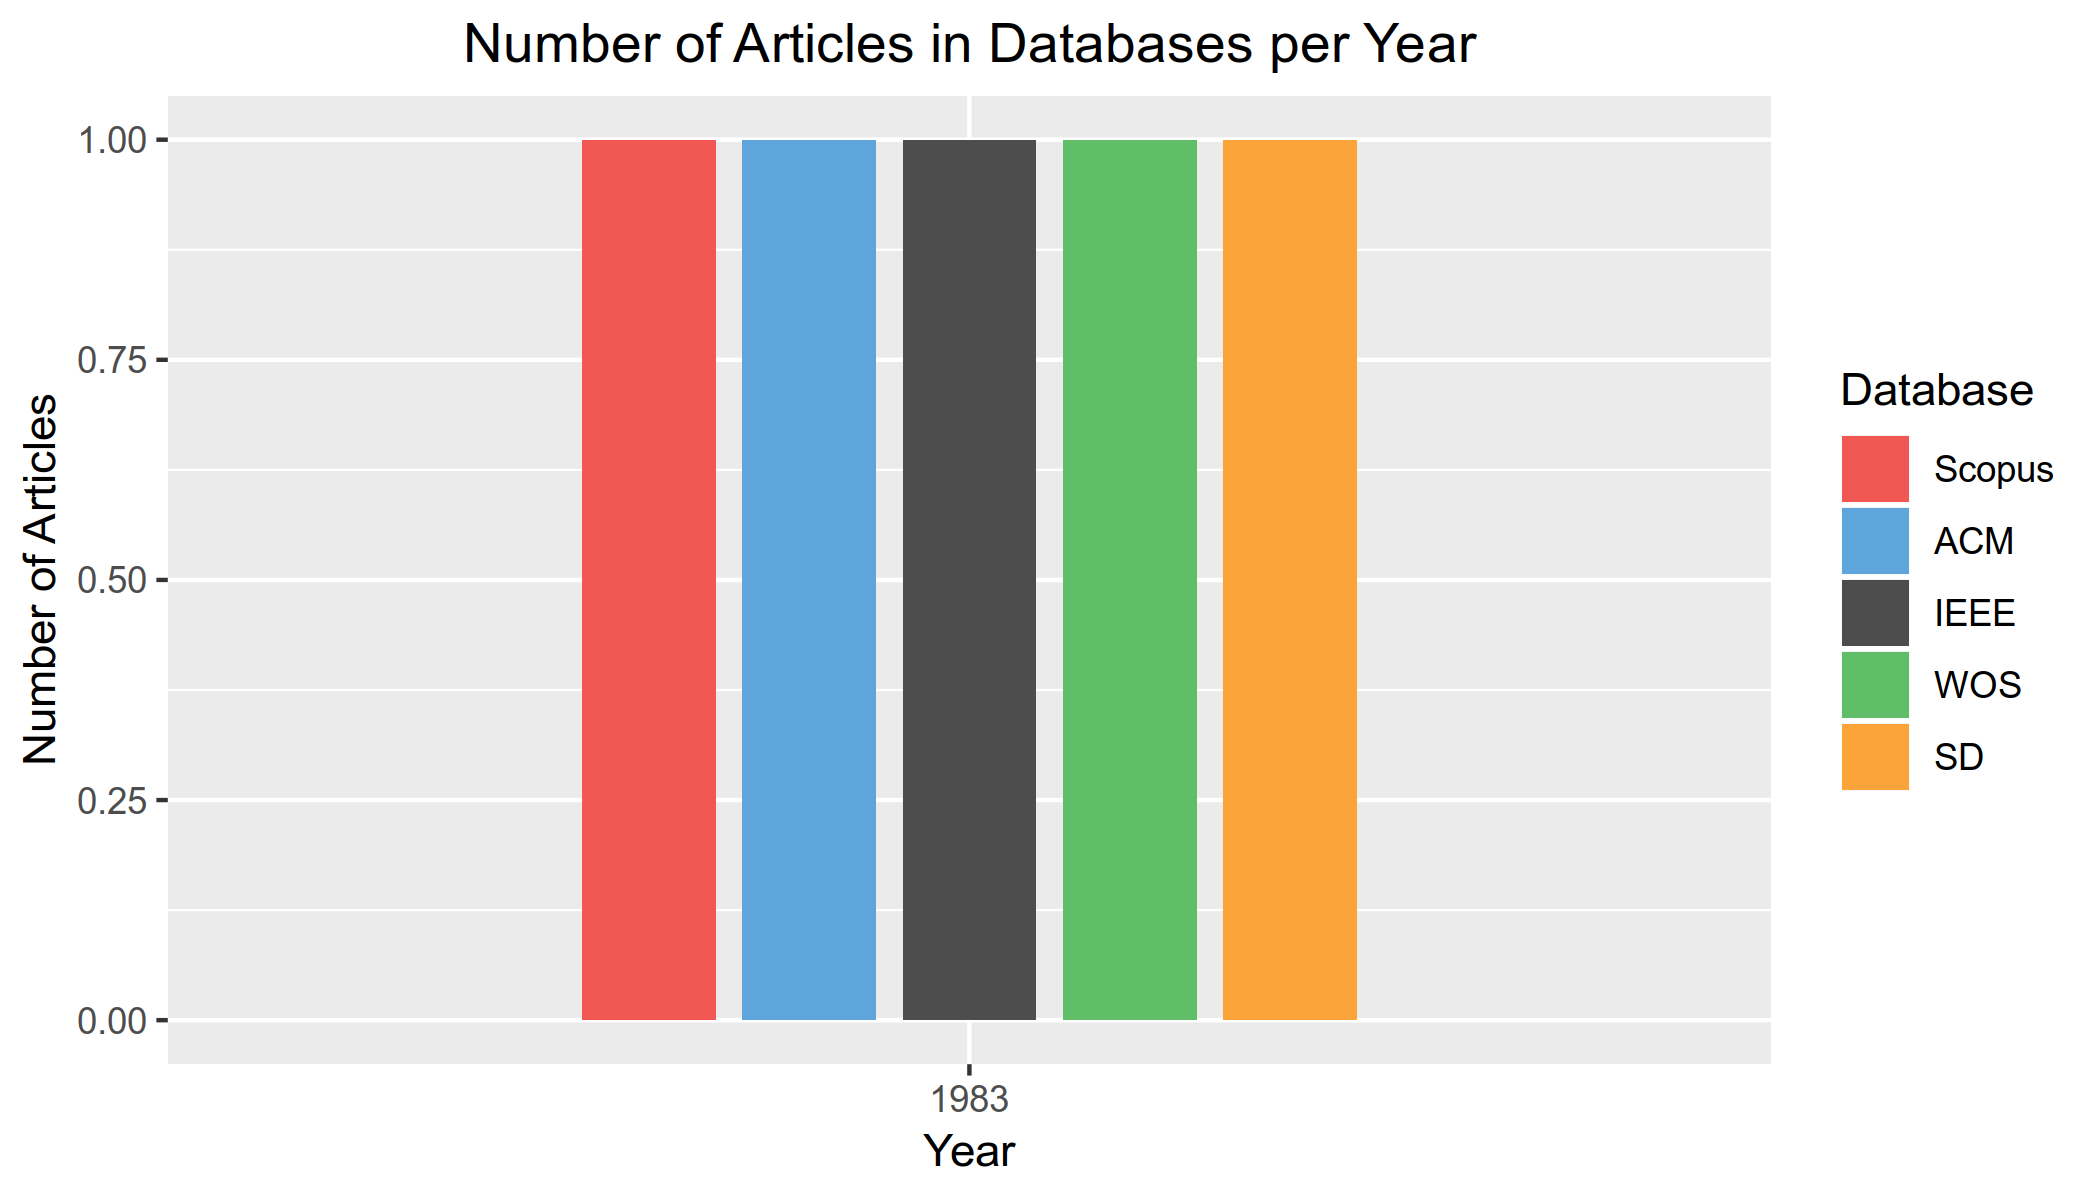
\includegraphics[width=\maxwidth]{figure/ImageFigureDatabases-1} 

\end{knitrout}
 	\caption{Number of articles in databases per year}\label{fig:databases}
 \end{figure}
 
 \begin{figure}[tb]
 	\centering
\begin{knitrout}
\definecolor{shadecolor}{rgb}{0.969, 0.969, 0.969}\color{fgcolor}
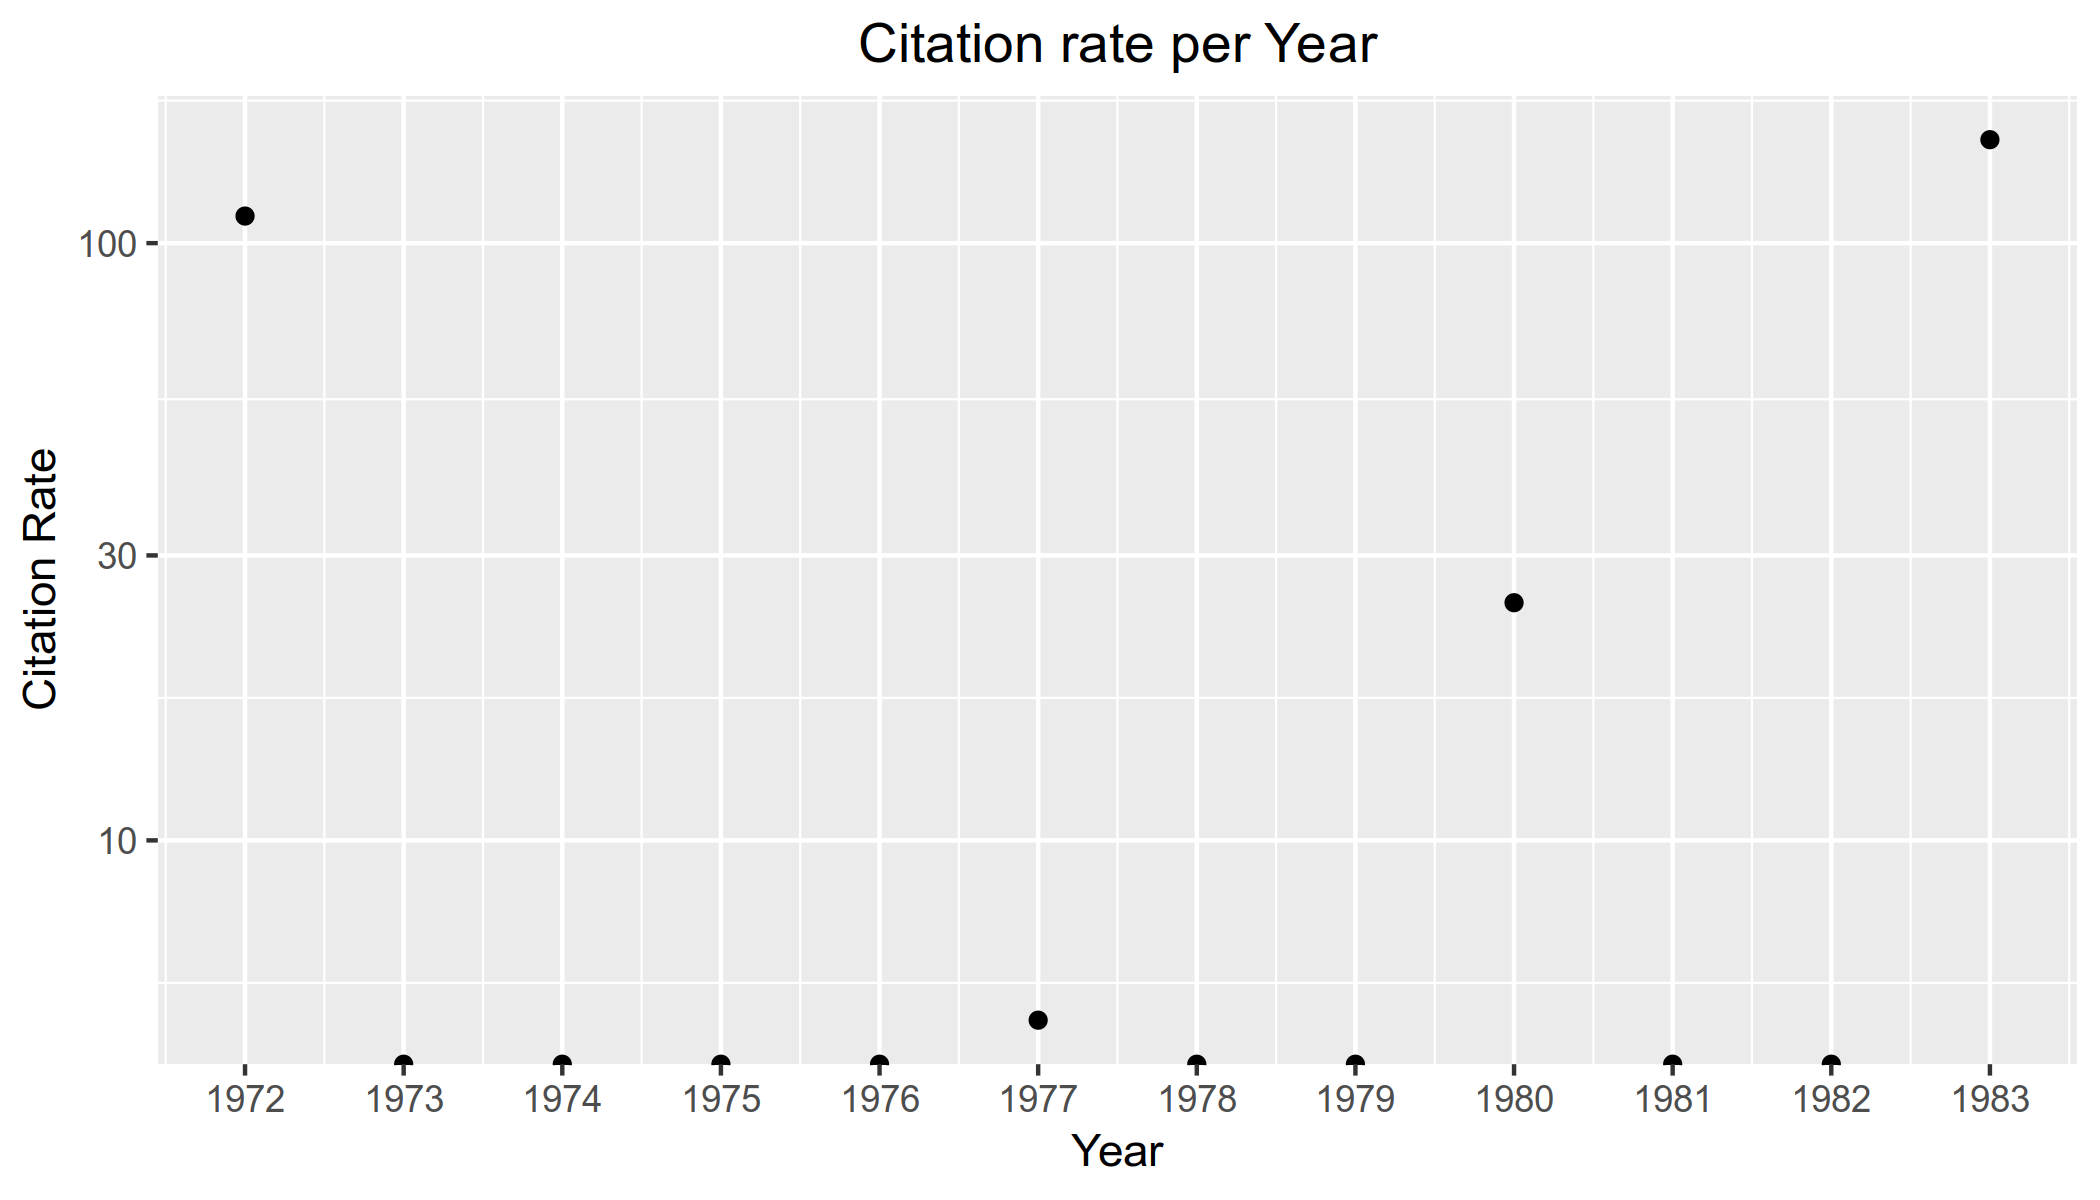
\includegraphics[width=\maxwidth]{figure/ImageFigureCitations-1} 

\end{knitrout}
 	\caption{Number of articles in databases per year}\label{fig:citations}
 \end{figure}
 
 
\subsection{Top authors}\label{sec:topAuthors}

Another way of finding relevant papers was to search for main authors in the field. A....

\begin{table} [bt]
	\centering
	\caption{Authors with most articles in SLR and most citations} \label{tbl:topAuthors}
	\rowcolors{2}{gray!6}{white}
	\begin{tabular}{l c c l} 
		\toprule
		& \textbf{Number of} & \textbf{Number of top} & \\
		\textbf{Author} & \textbf{articles} & \textbf{cited articles} & \textbf{Articles}\\ 
		\midrule 
		J, J         & 7 & 3 & \cite{ryan1991motivational} \\
		C, C   & 6 & 2 & \cite{ryan1991motivational}          \\
		\bottomrule
	\end{tabular}
\end{table}

\section{Research constraints}\label{sec:researchConstraints}

\chapter{Similarity detection tools}\label{ch:detectionTools}

    

\begin{table} [bt] 
	\centering 
	\caption{JPlag-java and SIM-java calibration dataset similarities} 
	\label{tbl:simJplagOptimalParamsCalibDataset} 
	\rowcolors{2}{gray!6}{white} 
	\begin{tabular}{l r r | r r} 
		\hiderowcolors 
		\toprule 
		& \multicolumn{4}{c}{\textbf{Similarity}} \\ 
		\cmidrule(l{2pt}r{2pt}){2-5} 
		& \multicolumn{2}{c}{\textbf{Java version}} & \multicolumn{2}{c}{\textbf{Text version}} \\ 
		\cmidrule(l{2pt}r{2pt}){2-3} \cmidrule(l{2pt}r{2pt}){4-5} 
		& \multicolumn{1}{c}{\textbf{JPlag}} &  \multicolumn{1}{c}{\textbf{SIM}} & \multicolumn{1}{c}{\textbf{JPlag}} &  \multicolumn{1}{c}{\textbf{SIM}}  \\ 
		\multicolumn{1}{c}{\textbf{Case name}} & \multicolumn{1}{c}{\textbf{(t=3)}} &  \multicolumn{1}{c}{\textbf{(r=22)}} & \multicolumn{1}{c}{\textbf{(t=8)}} &  \multicolumn{1}{c}{\textbf{(r=4)}}  \\ 
		\showrowcolors 
		\midrule 
		manual - 0\% example A             &  10.0 &   0.0 &   0.0 &   6.0\\  
		manual - 0\% example B             &  11.4 &   0.0 &   0.0 &   2.3\\  
		manual - 50\% Copy               &  64.1 &  58.5 &  40.7 &  56.5\\ 
		manual - 50\% Simple Obfuscation   &  67.5 &  67.0 &  48.8 &  64.0\\ 
		manual - 50\% Complex Obfuscation  &  64.1 &  58.0 &  39.9 &  57.0\\ 
		manual - 100\% Copy                & 100.0 & 100.0 &  99.7 & 100.0\\ 
		manual - 100\% Simple Obfuscation  &  98.3 & 100.0 &  96.7 & 100.0\\ 
		manual - 100\% Complex Obfuscation &  84.8 &  92.5 &  79.1 &  98.5\\ 
		SOCO 0 - N - (084-258)             &  45.7 &  14.5 &   0.0 &   4.7\\ 
		SOCO 1 - N - (000-001)             &  22.1 &   7.5 &   4.1 &  30.6\\ 
		SOCO 2 - N - (002-003)             &  28.9 &   0.0 &   4.0 &  10.2\\ 
		SOCO 3 - P - (003-004)             &  77.6 &  54.0 &  49.6 &  61.5\\ 
		SOCO 4 - P - (107-112)             & 100.0 & 100.0 &  33.3 &  75.0\\ 
		SOCO 5 - N - (052-077)             &  50.0 &   0.0 &   4.2 &  17.5\\ 
		SOCO 6 - N - (011-037)             &  38.5 &   0.0 &   0.0 &   3.0\\ 
		SOCO 7 - P - (062-064)             &  87.4 &  85.5 &  77.7 &  85.5\\ 
		SOCO 8 - N - (144-192)             &  57.1 &   1.0 &   0.0 &  15.3\\ 
		SOCO 9 - N - (037-093)             &  41.4 &   0.0 &   0.0 &  12.0\\ 
		\bottomrule 
		\hiderowcolors 
		\multicolumn{5}{l}{\footnotesize \textit{Note: }}\\ 
		\multicolumn{5}{l}{\footnotesize N in the case name marks a non-plagiarised case}\\ 
		\multicolumn{5}{l}{\footnotesize P in the case name marks a plagiarised case}\\ 
	\end{tabular} 
\end{table} 

\begin{table} [bt] 
	\centering 
	\caption{SIM-java calibrated with JPlag-java as base tool $^a$ } 
	\label{tbl:JPlagSIMJavaDiffs}  

\begin{threeparttable}
\begin{tabular}{ccr}
\toprule
\multicolumn{1}{c}{\textbf{JPlag-java (t)}} & \multicolumn{1}{c}{\textbf{SIM -java (r - best)}} & \multicolumn{1}{c}{\textbf{CDS}}\\
\midrule
\rowcolor{gray!6}  1 & 5 & 6\\
2 & 6 & 7\\
\rowcolor{gray!6}  3 & 7 & 8\\
4 & 8 & 9\\
\rowcolor{gray!6}  5 & 9 & 9\\
6 & 10 & 7\\
\rowcolor{gray!6}  7 & 11 & 8\\
8 & 12 & 9\\
\rowcolor{gray!6}  \textbf{9} & \textbf{13} & \textbf{10}\\
10 & 14 & 10\\
\rowcolor{gray!6}  11 & 15 & 8\\
12 & 16 & 9\\
\rowcolor{gray!6}  13 & 17 & 10\\
14 & 18 & 11\\
\rowcolor{gray!6}  15 & 19 & 11\\
\bottomrule
\end{tabular}
\begin{tablenotes}
\item[a] Footnote
\end{tablenotes}
\end{threeparttable}


\end{table} 



\chapter{Comparison measures}\label{ch:measures}
\lipsum[1-4]

\ldots

Performance Index is calculated as 
\[Performance\_index=D_{max}*\frac{1}{(tp+fn)*(1-P_L)}\] 
\begin{center}
	\centering or 
\end{center} 
\[Performance\_Index=MAX_{1-esm}\Bigg(\Big(tp_{@esm}-esm*\frac{tp+fn}{\frac{N}{2}}\Big)*
					\frac{1}{(tp+fn)*(1-\frac{tp+fn}{\frac{N}{2}})}\Bigg)\]
where: N is number of submissions; tp – true positive essential matches, fn – false negative essential matches; esm is number of essential matches; tp@esm – true positives essential matches at the number of essential matches.

\section{Precision, Recall and F-beta}\label{sec:PRF1}

Precision and Recall are calculated as follows: 
\[P = \frac{tp}{tp+fp}, \in [0,1] \ \ \ \ \ R = \frac{tp}{tp+fn}, \in [0,1] \]

F-beta is calculated as follows: 
\[F_\beta = \frac{(\beta^2 + 1) * P * R}{(\beta^2 * P) + R}, \in [0,1]\]

\chapter{Preprocessing techniques}\label{ch:preporcessing}

    


\begin{table}
	\centering
	\caption{JPlag-text and SIM-text PPTest result} \label{tbl:resultsPPTestText}

\begin{tabular}{lrrrr|>{}rrrr}
\toprule
\multicolumn{1}{c}{\textbf{ }} & \multicolumn{4}{c}{\textbf{JPlag Text}} & \multicolumn{4}{c}{\textbf{SIM Text}} \\
\cmidrule(l{3pt}r{3pt}){2-5} \cmidrule(l{3pt}r{3pt}){6-9}
\multicolumn{1}{c}{\textbf{Technique Name}} & \multicolumn{1}{c}{\textbf{E1}} & \multicolumn{1}{c}{\textbf{E2}} & \multicolumn{1}{c}{\textbf{E3}} & \multicolumn{1}{c}{\textbf{E4}} & \multicolumn{1}{c}{\textbf{E1}} & \multicolumn{1}{c}{\textbf{E2}} & \multicolumn{1}{c}{\textbf{E3}} & \multicolumn{1}{c}{\textbf{E4 }}\\
\midrule
\rowcolor{gray!6}  No Preprocessing & 1 & 2 & 3 & 4 & 5 & 6 & 7 & 8\\
\addlinespace[0.3em]
\multicolumn{9}{l}{\textbf{Techniques}}\\
\textbf{\hspace{1em}Remove Comments (RC)} & \textbf{2} & \textbf{3} & \textbf{4} & \textbf{5} & \textbf{6} & \textbf{7} & \textbf{8} & \textbf{9}\\
\rowcolor{gray!6}  \hspace{1em}Remove White Spaces (RWS) & 3 & 4 & 5 & 6 & 7 & 8 & 9 & 10\\
\hspace{1em}Normalise (NOR) & 4 & 5 & 6 & 7 & 8 & 9 & 10 & 11\\
\rowcolor{gray!6}  \textbf{\hspace{1em}Common Code Remove (CCR)} & \textbf{5} & \textbf{6} & \textbf{7} & \textbf{8} & \textbf{9} & \textbf{10} & \textbf{11} & \textbf{12}\\
\textbf{\hspace{1em}Template Exlusion (TE)} & \textbf{6} & \textbf{7} & \textbf{8} & \textbf{9} & \textbf{10} & \textbf{11} & \textbf{12} & \textbf{13}\\
\rowcolor{gray!6}  \addlinespace[0.3em]
\multicolumn{9}{l}{\textbf{Combinations}}\\
\textbf{\hspace{1em}All (TE-RC-CCR-NOR-RWS)} & \textbf{7} & \textbf{8} & \textbf{9} & \textbf{10} & \textbf{11} & \textbf{12} & \textbf{13} & \textbf{14}\\
\hspace{1em}RC-NOR-RWS & 8 & 9 & 10 & 11 & 12 & 13 & 14 & 15\\
\rowcolor{gray!6}  \hspace{1em}NOR-RC & 9 & 10 & 11 & 12 & 13 & 14 & 15 & 16\\
\hspace{1em}RC-NOR & 10 & 11 & 12 & 13 & 14 & 15 & 16 & 17\\
\rowcolor{gray!6}  \textbf{\hspace{1em}TE-CCR} & \textbf{11} & \textbf{12} & \textbf{13} & \textbf{14} & \textbf{15} & \textbf{16} & \textbf{17} & \textbf{18}\\
\bottomrule
\end{tabular}


\end{table}

\chapter{Result analysis}\label{ch:analysis}

    

This Chapter provides the complete results of this research. Before the results are presented there is a description of some preparations that are important for the analysis.

\section{SOCO dataset analysis}

\begin{table} [bt]
	\centering
	\caption{SOCO dataset structure for experiment} \label{tbl:socoSubsetStructure}
	\rowcolors{2}{gray!6}{white}
	\begin{tabular}{c | c c | r r r r} 
		\toprule
		&  \multicolumn{2}{c}{\textbf{Assignment}} & \multicolumn{4}{c}{\textbf{Number of}} \\
		\cmidrule(l{3pt}r{3pt}){2-3} \cmidrule(l{3pt}r{3pt}){4-7}
		\textbf{Collection} & \textbf{original} & \textbf{new} & \multicolumn{1}{c}{\textbf{Files}} & \multicolumn{1}{c}{\textbf{Plagiarized files}} & \multicolumn{1}{c}{\textbf{Matches}} & \multicolumn{1}{c}{\textbf{Plagiarised matches}} \\ 
		\midrule 
		 	Test & A1 & D1 & 188 &  86 & 17,578&  54  \\
		 	Test & A2 & D2 & 175 &  75 & 15,225&  47  \\
		 	Test & B1 & D3 & 218 & 124 & 23,653&  73  \\
		\bottomrule
	\end{tabular}
\end{table}

\subsubsection{Preparation for statistical analysis}

The full model used was: 
\begin{gather*}
lmer(F1 \sim Tool + Technique + Tool:Technique + \notag\\
             (1 | Participant) + (1 | Tool:Participant) + (1 | Technique:Participant), \notag\\ 
     data = SOCO.Dn, REML = FALSE)
\end{gather*}
The null model was: 
\begin{gather*}
lmer(F1 \sim (1 | Participant) + (1 | Tool:Participant) + (1 | Technique:Participant), \notag\\
     data = SOCO.Dn, REML = FALSE)
\end{gather*}

The full model for the simple effects analysis was:
\begin{gather*}
lmer(F1 \sim ToolTechniqueCombo + \notag\\
             (1 | Participant) + (1 | Tool:Participant) + (1 | Technique:Participant), \notag\\ 
     data = SOCO.Dn, REML = FALSE)
\end{gather*} 
and the null model was the same as written above. Recall that the term \textit{Participant} represents one subset assignment (e.g., Dn-1, Dn-2, Dn-3, etc.) from the D1, D2, D3 or D4 group of assignments.

To perform the bootstrap hypothesis testing the function \textit{boot} from package \textit{boot} was used, and to get confidence intervals the function \textit{boot.ci} from package \textit{boot} was used or function \textit{bootMer} from the \textit{lme4} package. Models were compared using the \textit{PBmodcomp} function from the \textit{pbkrtest} package. The full list of packages used in R is presented in Appendix \ref{apx:rPackages}.

\subsection{Results for D1 assignments}

    

D1 assignments are created from the A1 assignment in the \gls{SOCO} dataset. 

\begin{figure}
	\centering 
\begin{knitrout}
\definecolor{shadecolor}{rgb}{0.969, 0.969, 0.969}\color{fgcolor}
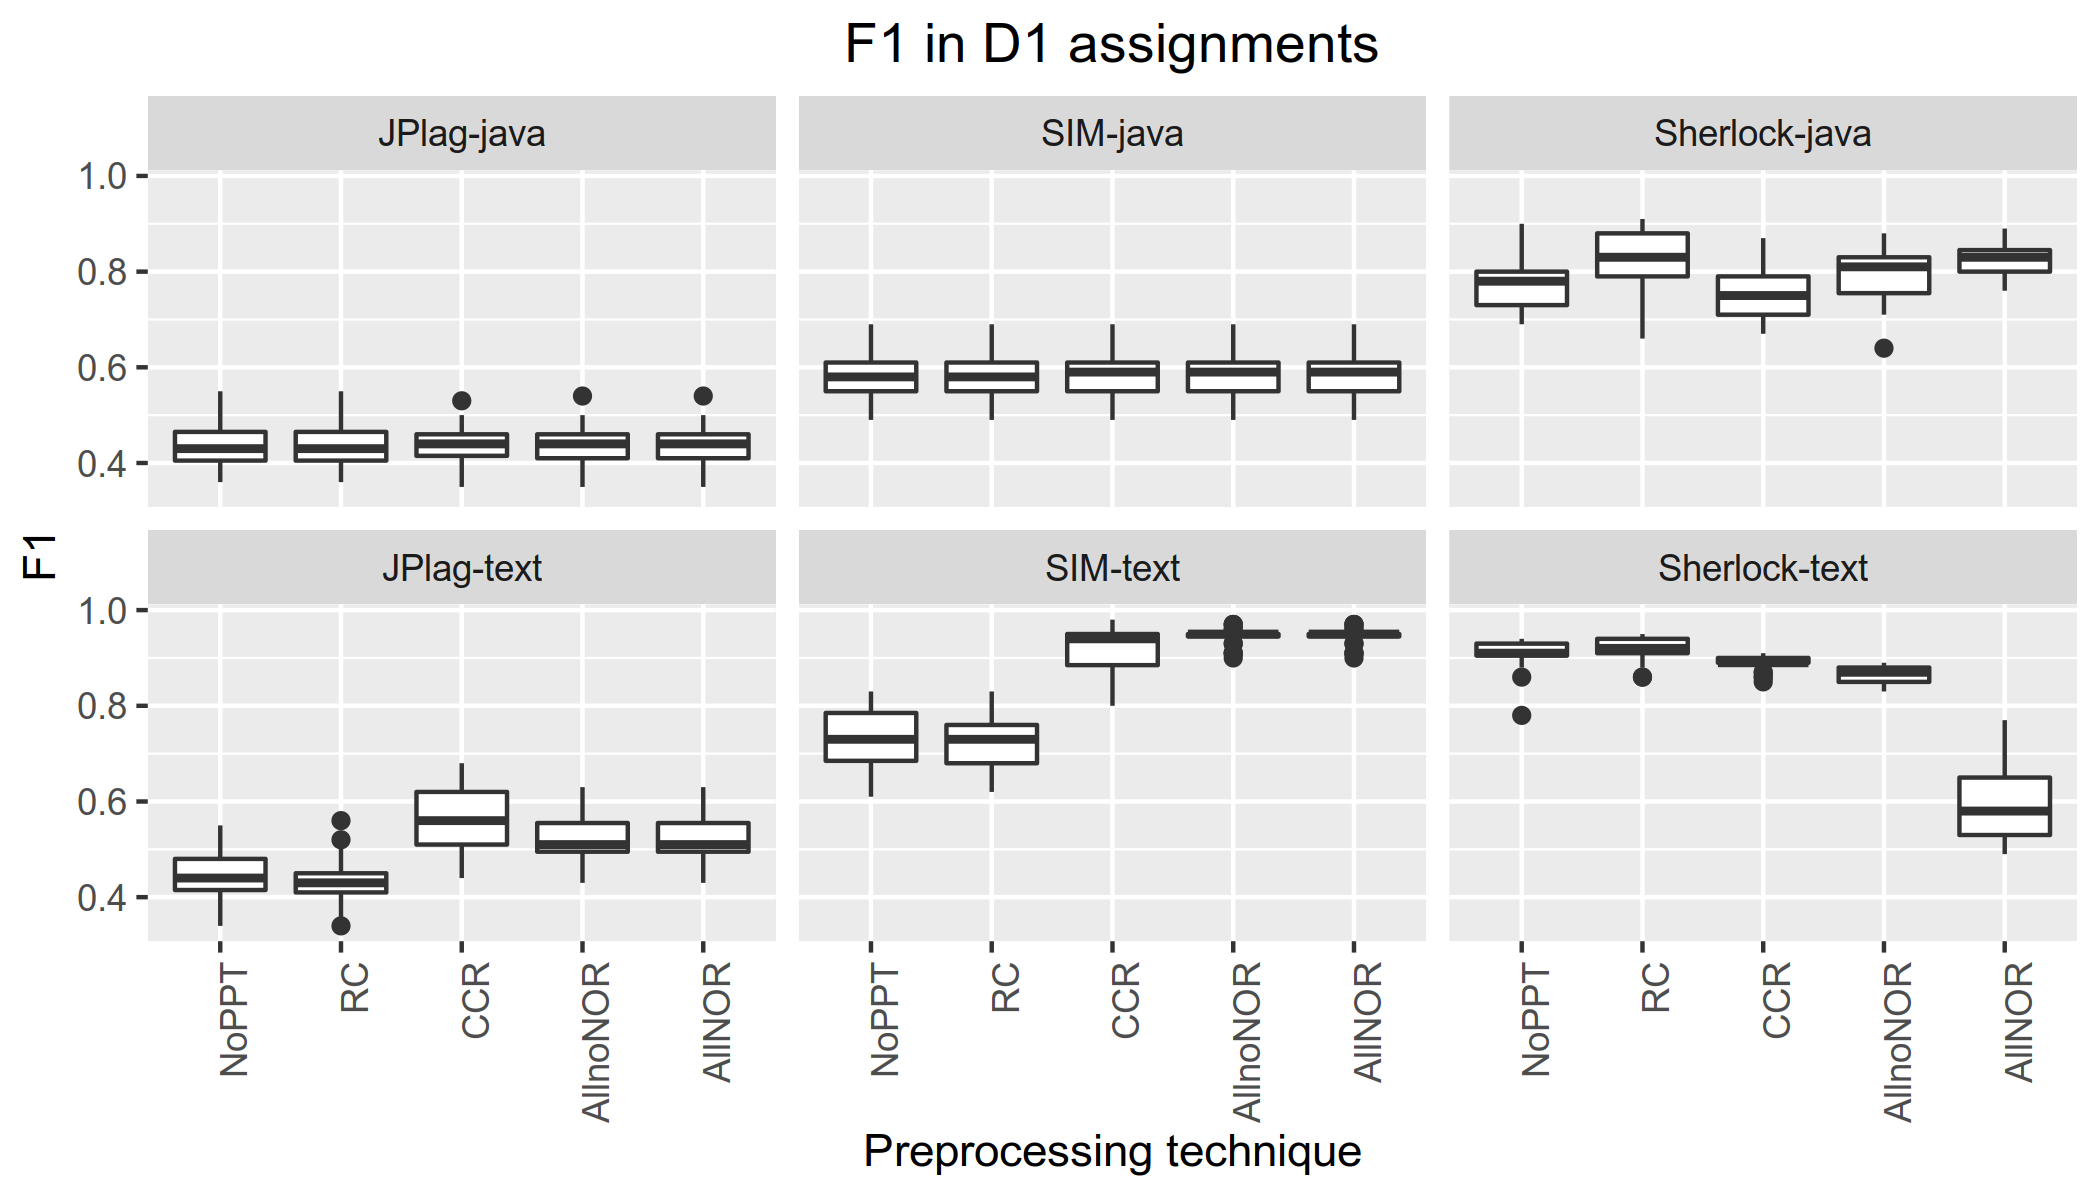
\includegraphics[width=\maxwidth]{figure/FigureBoxPlotD13IRQ-1} 

\end{knitrout}
	\caption{F1 score for SOCO D1 assignment with 3*IRQ}\label{fig:FigureBoxPlotD13IRQ}
\end{figure}

\begin{figure}
	\centering
    \minipage{0.32\textwidth}
\begin{knitrout}
\definecolor{shadecolor}{rgb}{0.969, 0.969, 0.969}\color{fgcolor}
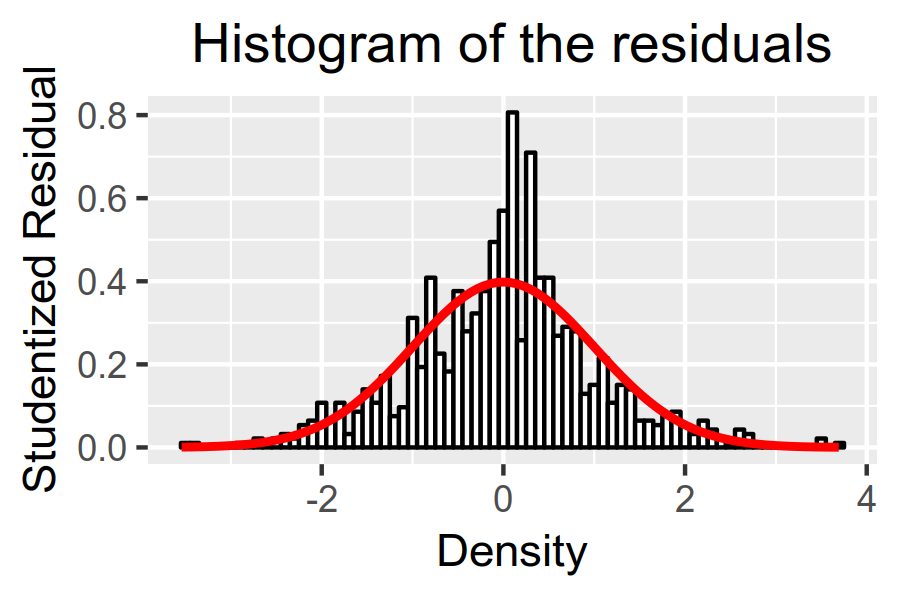
\includegraphics[width=\maxwidth]{figure/Figure-Histogram-D1-1} 

\end{knitrout}
%      \caption{A really Awesome Image}\label{fig:awesome_image1}
    \endminipage\hfill 
    \minipage{0.32\textwidth}
\begin{knitrout}
\definecolor{shadecolor}{rgb}{0.969, 0.969, 0.969}\color{fgcolor}
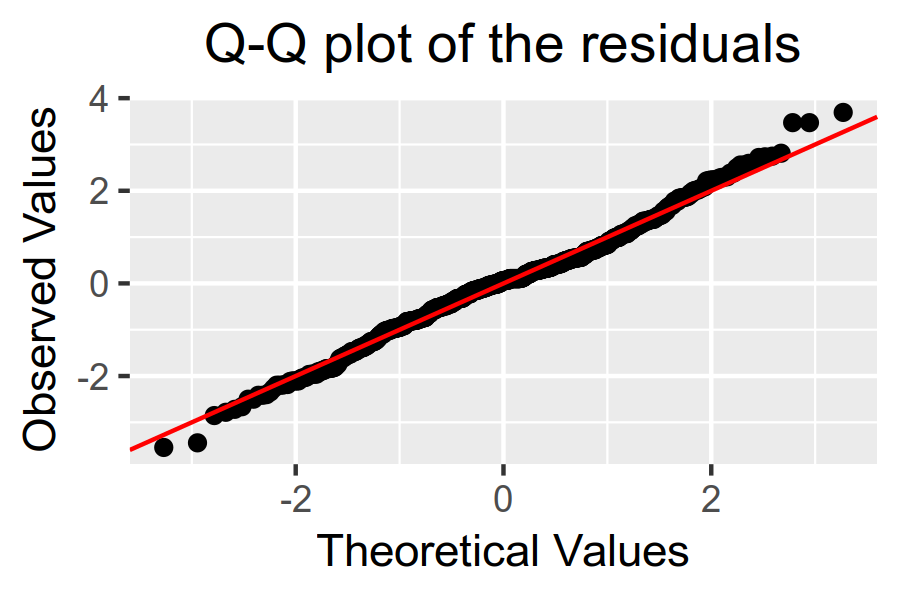
\includegraphics[width=\maxwidth]{figure/Figure-Q-Q-D1-1} 

\end{knitrout}
%      \caption{A really Awesome Image}\label{fig:awesome_image2}
    \endminipage\hfill 
    \minipage{0.32\textwidth}%
\begin{knitrout}
\definecolor{shadecolor}{rgb}{0.969, 0.969, 0.969}\color{fgcolor}
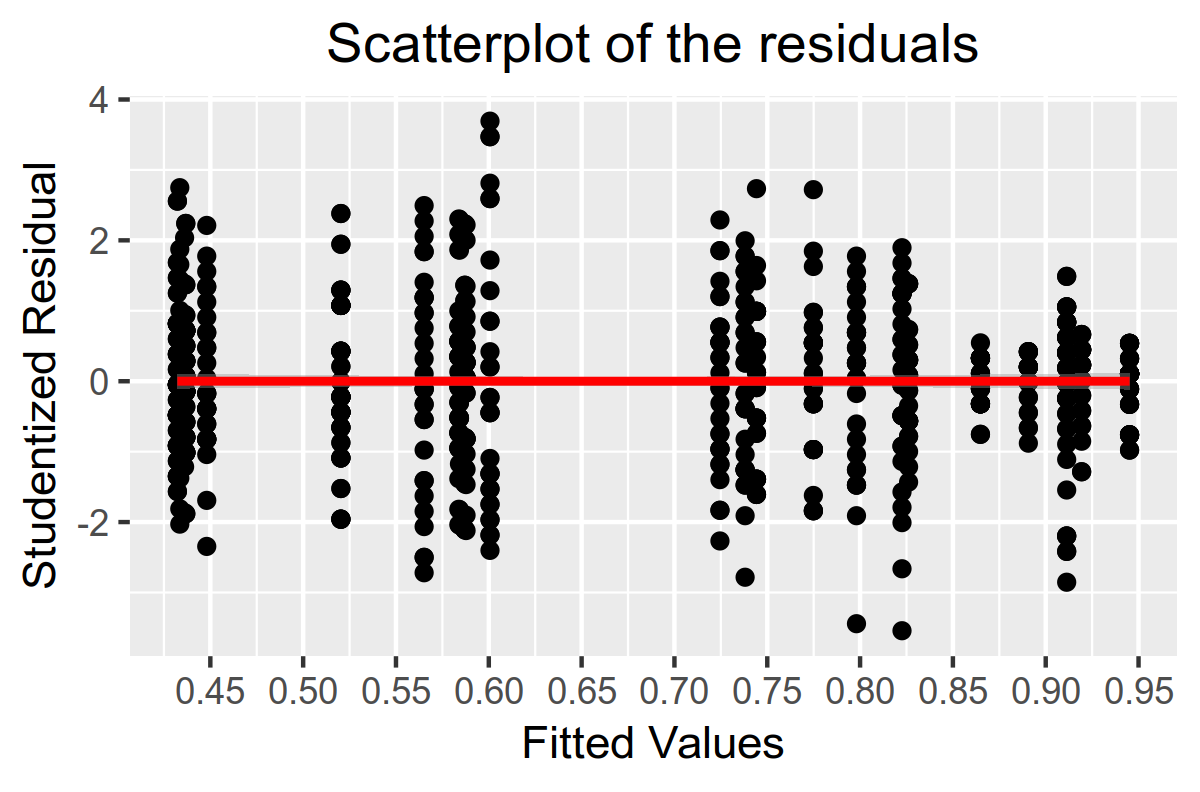
\includegraphics[width=\maxwidth]{figure/Figure-Scatter-D1-1} 

\end{knitrout}
%      \caption{A really Awesome Image}\label{fig:awesome_image3}
    \endminipage
	\caption{D1 assignments - residuals}\label{fig:normalityD1F1}
\end{figure}

To confirm ...

\begin{table}
  \centering 
  \caption{ANOVA results for SOCO D1}\label{tbl:anovaSOCOD1}

\begin{tabular}{lrrrrrrr}
\toprule
\multicolumn{1}{c}{\textbf{ }} & \multicolumn{1}{c}{\textbf{Sum Sq}} & \multicolumn{1}{c}{\textbf{Mean Sq}} & \multicolumn{1}{c}{\textbf{NumDF}} & \multicolumn{1}{c}{\textbf{DenDF}} & \multicolumn{1}{c}{\textbf{F value}} & \multicolumn{1}{c}{\textbf{Pr(>F)}} & \multicolumn{1}{c}{\textbf{p.boot}}\\
\midrule
\rowcolor{gray!6}  Tool & 4.07 & 0.814 & 5 & 155 & 818.0 & 0.0000 & 0.0001\\
Technique & 0.34 & 0.085 & 4 & 124 & 85.9 & 0.0000 & 0.0001\\
\rowcolor{gray!6}  \textbf{Tool:Technique} & \textbf{3.95} & \textbf{0.198} & \textbf{20} & \textbf{620} & \textbf{198.7} & \textbf{0.0000} & \textbf{0.0001}\\
\bottomrule
\end{tabular}


\end{table}

Since ....

\begin{figure}
	\centering 

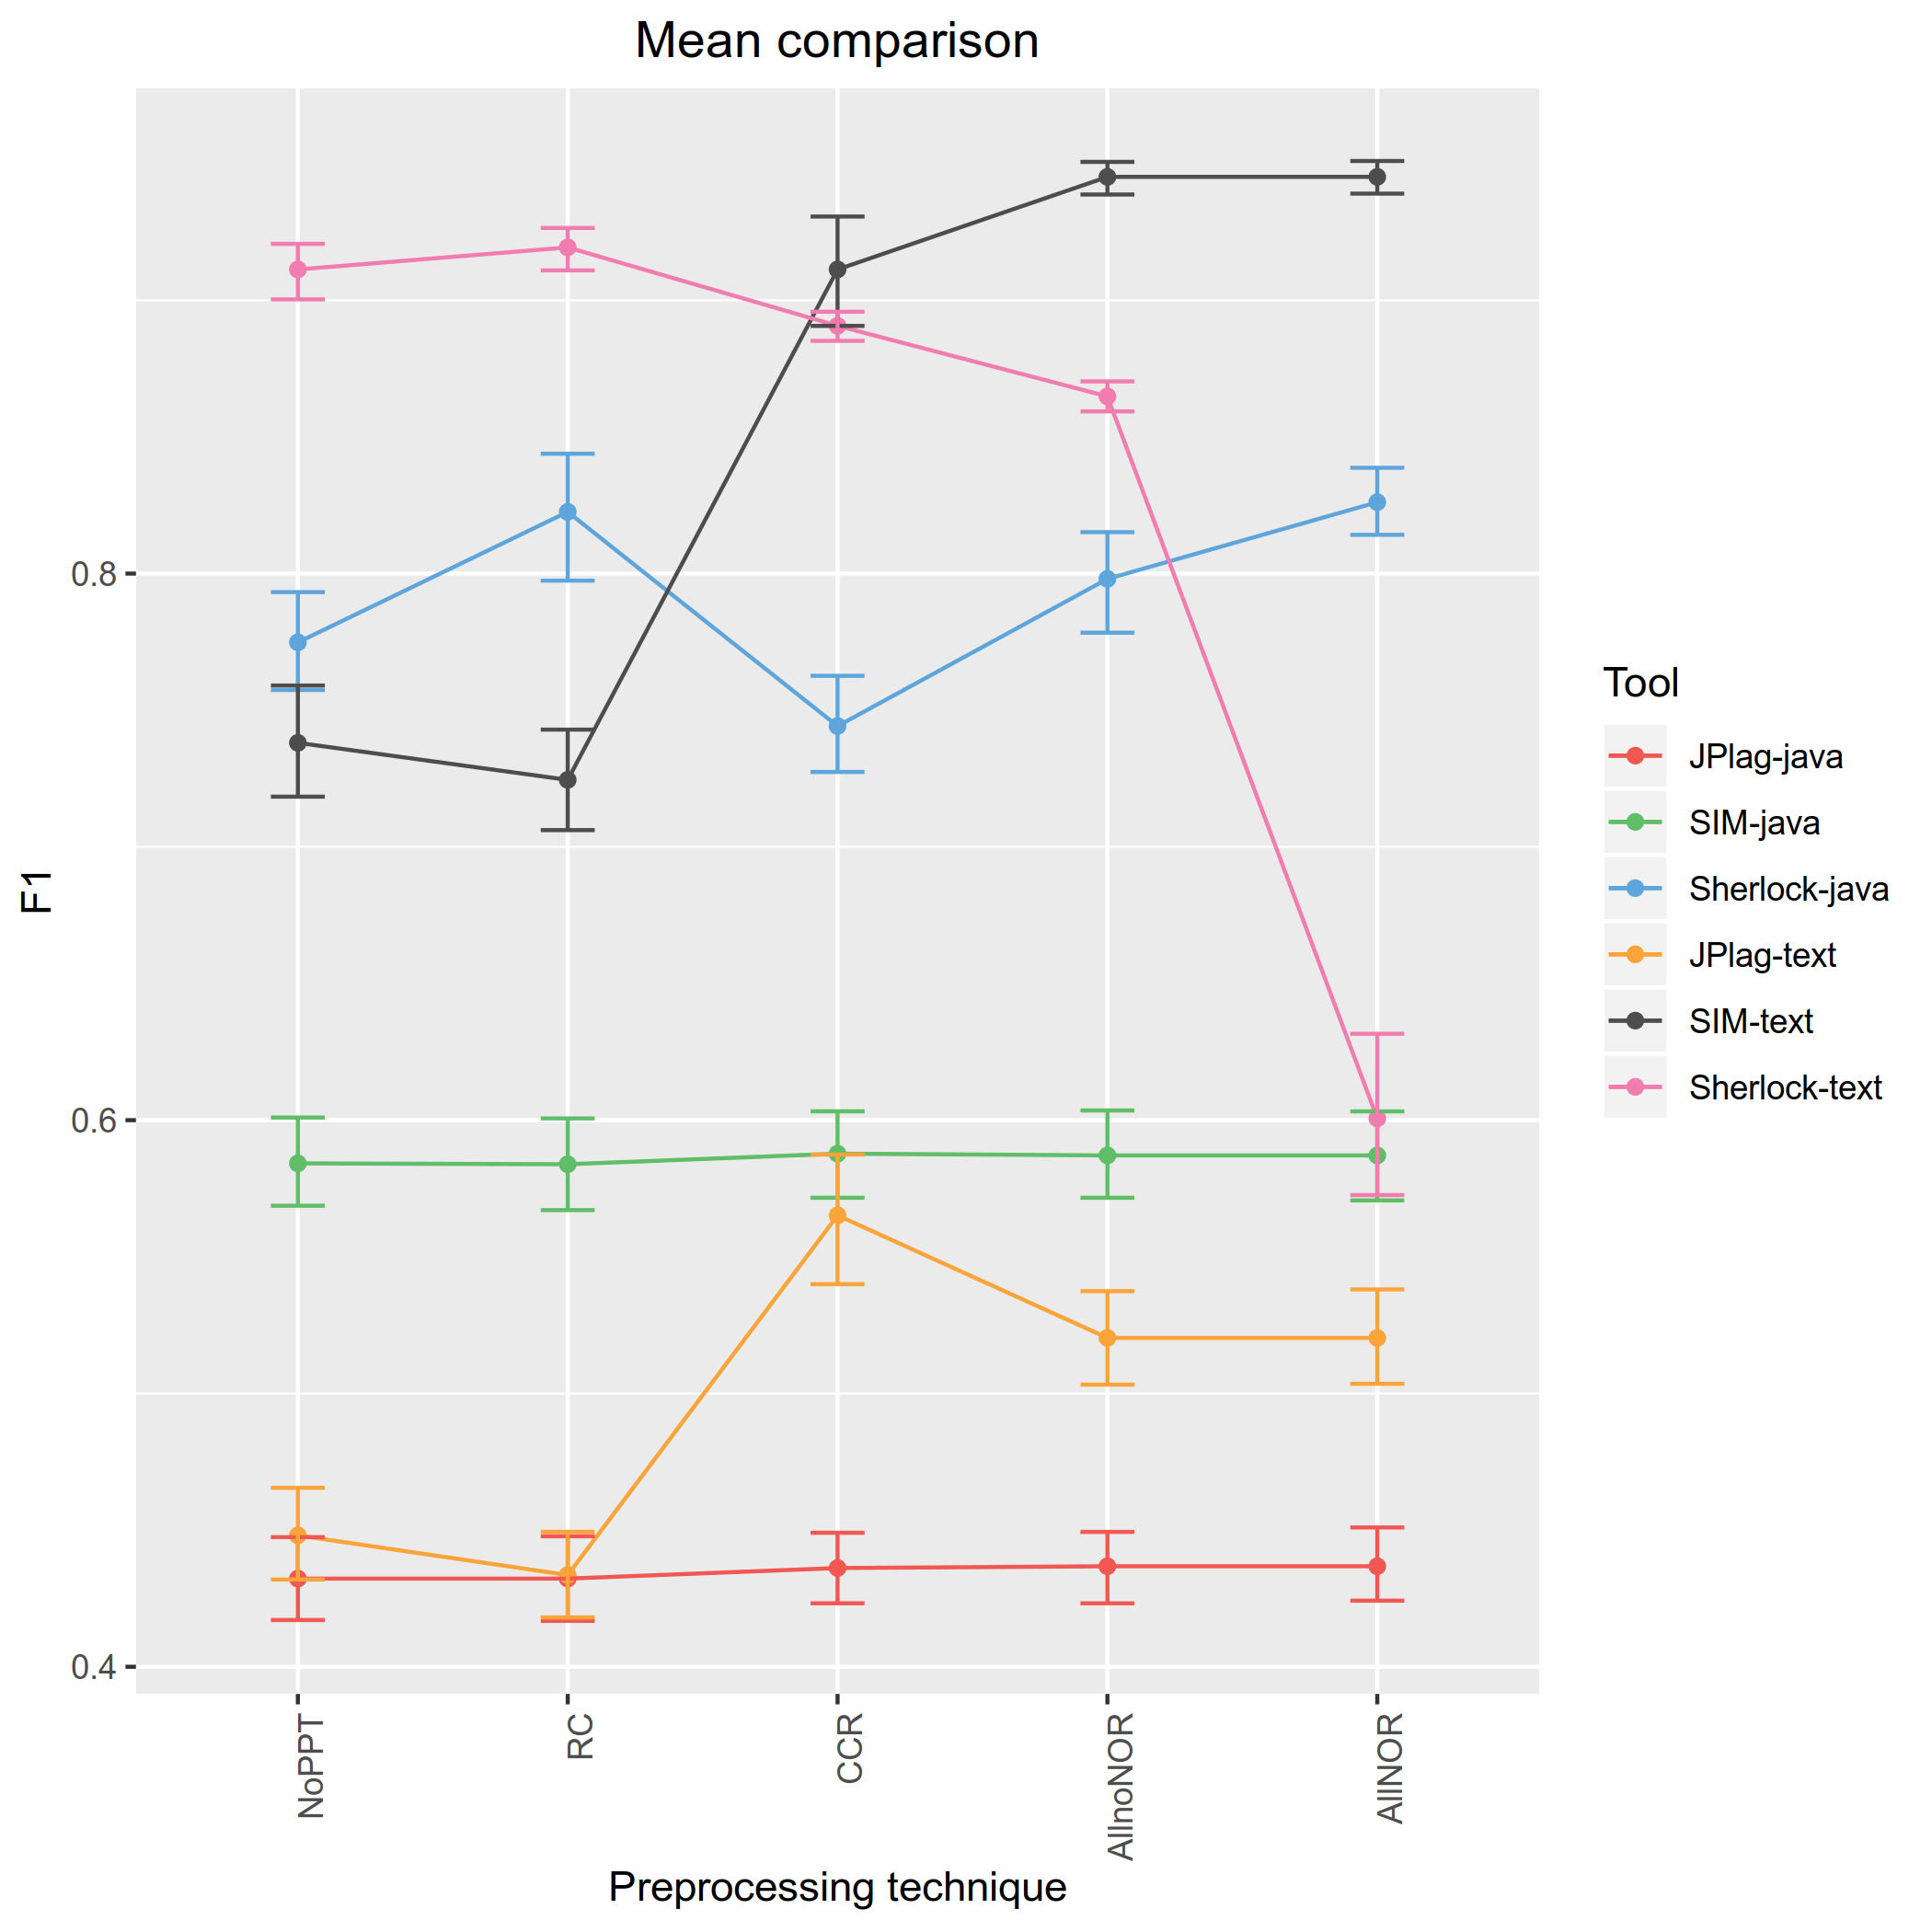
\includegraphics[width=\maxwidth]{figure/FigureMeanComparisonGraphSOCOD1-1} 

	\caption{F1 mean comparison for SOCO D1}\label{fig:meanComparisonSOCOD1}
\end{figure}

To (Table \ref{tbl:anovaSOCOD1}).

Figure \ref{fig:meanComparisonSOCOD1} .

By looking at Figure \ref{fig:meanComparisonSOCOD1} .

\begin{table}
  \centering 
  \caption{Contrasts results for SOCO D1}\label{tbl:coefficientsSOCOD1} 

\begin{threeparttable}
\begin{tabular}{rrrrrrr}
\toprule
\multicolumn{1}{c}{\textbf{Name}} & \multicolumn{1}{c}{\textbf{Estimate}} & \multicolumn{1}{c}{\textbf{SE}} & \multicolumn{1}{c}{\textbf{df}} & \multicolumn{1}{c}{\textbf{t.value}} & \multicolumn{1}{c}{\textbf{Pr(>|t|)}} & \multicolumn{1}{c}{\textbf{p.boot}}\\
\midrule
\rowcolor{gray!6}  \textbf{(Intercept)} & 0.667 & 0 & 31 & 228.7363 & 0.0000 & \textbf{0.0001}\\
\textbf{Tool.TextvsJava} & -0.062 & 0 & 155 & -23.7553 & 0.0000 & \textbf{0.0001}\\
\rowcolor{gray!6}  \textbf{TT.SHvsOthers} & -0.054 & 0 & 155 & -20.6218 & 0.0000 & \textbf{0.0001}\\
\textbf{TJ.SHvsOthers} & -0.094 & 0 & 155 & -35.9487 & 0.0000 & \textbf{0.0001}\\
\rowcolor{gray!6}  \textbf{TT.SIMvsJPlag} & -0.178 & 0 & 155 & -39.1278 & 0.0000 & \textbf{0.0001}\\
\textbf{TJ.SIMvsJPlag} & -0.076 & 0 & 155 & -16.6443 & 0.0000 & \textbf{0.0001}\\
\rowcolor{gray!6}  \textbf{NoPPTvsPPT} & 0.005 & 0 & 124 & 8.8276 & 0.0000 & \textbf{0.0001}\\
SinglevsCombo & 0.001 & 0 & 124 & 0.5975 & 0.5513 & 0.8008\\
\rowcolor{gray!6}  \textbf{RCvsCCR} & 0.018 & 0 & 124 & 10.8250 & 0.0000 & \textbf{0.0001}\\
\textbf{AnoNvsAN} & -0.020 & 0 & 124 & -11.6699 & 0.0000 & \textbf{0.0001}\\
\hline
\rowcolor{gray!6}  \textbf{Tool.TextvsJava:NoPPTvsPPT} & -0.003 & 0 & 620 & -5.4427 & 0.0000 & \textbf{0.0001}\\
\textbf{TT.SHvsOthers:NoPPTvsPPT} & 0.013 & 0 & 620 & 25.1444 & 0.0000 & \textbf{0.0001}\\
\rowcolor{gray!6}  \textbf{TJ.SHvsOthers:NoPPTvsPPT} & -0.001 & 0 & 620 & -2.5992 & 0.0096 & \textbf{0.0073}\\
\textbf{TT.SIMvsJPlag:NoPPTvsPPT} & -0.008 & 0 & 620 & -9.1208 & 0.0000 & \textbf{0.0001}\\
\rowcolor{gray!6}  TJ.SIMvsJPlag:NoPPTvsPPT & 0.000 & 0 & 620 & 0.1080 & 0.9140 & 0.5662\\
Tool.TextvsJava:SinglevsCombo & 0.005 & 0 & 620 & 4.0800 & 0.0001 & 0.0221\\
\rowcolor{gray!6}  \textbf{TT.SHvsOthers:SinglevsCombo} & 0.041 & 0 & 620 & 35.5109 & 0.0000 & \textbf{0.0001}\\
\textbf{TJ.SHvsOthers:SinglevsCombo} & -0.004 & 0 & 620 & -3.8591 & 0.0001 & \textbf{0.0004}\\
\rowcolor{gray!6}  \textbf{TT.SIMvsJPlag:SinglevsCombo} & -0.027 & 0 & 620 & -13.2677 & 0.0000 & \textbf{0.0001}\\
TJ.SIMvsJPlag:SinglevsCombo & 0.000 & 0 & 620 & 0.1611 & 0.8721 & 0.5987\\
\rowcolor{gray!6}  \textbf{Tool.TextvsJava:RCvsCCR} & -0.030 & 0 & 620 & -18.3619 & 0.0000 & \textbf{0.0001}\\
\textbf{TT.SHvsOthers:RCvsCCR} & 0.031 & 0 & 620 & 19.1510 & 0.0000 & \textbf{0.0001}\\
\rowcolor{gray!6}  \textbf{TJ.SHvsOthers:RCvsCCR} & 0.014 & 0 & 620 & 8.3837 & 0.0000 & \textbf{0.0001}\\
\textbf{TT.SIMvsJPlag:RCvsCCR} & -0.014 & 0 & 620 & -4.8688 & 0.0000 & \textbf{0.0001}\\
\rowcolor{gray!6}  TJ.SIMvsJPlag:RCvsCCR & 0.000 & 0 & 620 & 0.0000 & 1.0000 & 0.5130\\
\textbf{Tool.TextvsJava:AnoNvsAN} & 0.024 & 0 & 620 & 14.8934 & 0.0000 & \textbf{0.0001}\\
\rowcolor{gray!6}  \textbf{TT.SHvsOthers:AnoNvsAN} & 0.044 & 0 & 620 & 26.9264 & 0.0000 & \textbf{0.0001}\\
\textbf{TJ.SHvsOthers:AnoNvsAN} & -0.005 & 0 & 620 & -2.8603 & 0.0044 & \textbf{0.0034}\\
\rowcolor{gray!6}  TT.SIMvsJPlag:AnoNvsAN & 0.000 & 0 & 620 & 0.0000 & 1.0000 & 0.5259\\
TJ.SIMvsJPlag:AnoNvsAN & 0.000 & 0 & 620 & 0.0000 & 1.0000 & 0.5265\\
\bottomrule
\end{tabular}
\begin{tablenotes}
\item \textit{Note: } 
\item TT - ToolText, TJ - ToolJava, SH - Sherlock, AnoN - AllnoNOR, AN - AllNOR
\end{tablenotes}
\end{threeparttable}


\end{table}

\begin{table}
	\centering 
	\caption{Simple effect analysis result for SOCO D1}\label{tbl:simpleEffectAnalysisSOCOD1}

\begin{threeparttable}
\begin{tabular}{rrrrrrr}
\toprule
\multicolumn{1}{c}{\textbf{Name}} & \multicolumn{1}{c}{\textbf{Estimate}} & \multicolumn{1}{c}{\textbf{SE}} & \multicolumn{1}{c}{\textbf{df}} & \multicolumn{1}{c}{\textbf{t.value}} & \multicolumn{1}{c}{\textbf{Pr(>|t|)}} & \multicolumn{1}{c}{\textbf{p.boot}}\\
\midrule
\rowcolor{gray!6}  \textbf{(Intercept)} & 0.667 & 0 & 31.0 & 228.7363 & 0.0000 & \textbf{0.0001}\\
\textbf{TextvsJava} & -0.062 & 0 & 155.0 & -23.7553 & 0.0000 & \textbf{0.0001}\\
\rowcolor{gray!6}  \textbf{TT.SHvsOthers} & -0.054 & 0 & 155.0 & -20.6218 & 0.0000 & \textbf{0.0001}\\
\textbf{TT.SIMvsJPlag} & -0.178 & 0 & 155.0 & -39.1278 & 0.0000 & \textbf{0.0001}\\
\rowcolor{gray!6}  \textbf{TJ.SHvsOthers} & -0.094 & 0 & 155.0 & -35.9487 & 0.0000 & \textbf{0.0001}\\
\textbf{TJ.SIMvsJPlag} & -0.076 & 0 & 155.0 & -16.6443 & 0.0000 & \textbf{0.0001}\\
\hline
\rowcolor{gray!6}  \textbf{TT.SH.NoPPTvsPPT} & -0.018 & 0 & 743.6 & -14.5161 & 0.0000 & \textbf{0.0001}\\
\textbf{TT.SH.SinglevsCombo} & -0.086 & 0 & 743.6 & -30.2497 & 0.0000 & \textbf{0.0001}\\
\rowcolor{gray!6}  \textbf{TT.SH.RCvsCCR} & -0.014 & 0 & 743.6 & -3.5650 & 0.0004 & \textbf{0.0003}\\
\textbf{TT.SH.AllnoNORvsAllNOR} & -0.132 & 0 & 743.6 & -32.8057 & 0.0000 & \textbf{0.0001}\\
\rowcolor{gray!6}  \textbf{TT.JPlag.NoPPTvsPPT} & 0.012 & 0 & 743.6 & 9.7027 & 0.0000 & \textbf{0.0001}\\
TT.JPlag.SinglevsCombo & 0.010 & 0 & 743.6 & 3.6821 & 0.0002 & 0.0453\\
\rowcolor{gray!6}  \textbf{TT.JPlag.RCvsCCR} & 0.066 & 0 & 743.6 & 16.3428 & 0.0000 & \textbf{0.0001}\\
TT.JPlag.AllnoNORvsAllNOR & 0.000 & 0 & 743.6 & 0.0000 & 1.0000 & 0.5204\\
\rowcolor{gray!6}  \textbf{TT.SIM.NoPPTvsPPT} & 0.029 & 0 & 743.6 & 22.5342 & 0.0000 & \textbf{0.0001}\\
\textbf{TT.SIM.SinglevsCombo} & 0.064 & 0 & 743.6 & 22.3474 & 0.0000 & \textbf{0.0001}\\
\rowcolor{gray!6}  \textbf{TT.SIM.RCvsCCR} & 0.093 & 0 & 743.6 & 23.1923 & 0.0000 & \textbf{0.0001}\\
TT.SIM.AllnoNORvsAllNOR & 0.000 & 0 & 743.6 & 0.0000 & 1.0000 & 0.5241\\
\rowcolor{gray!6}  TJ.SH.NoPPTvsPPT & 0.005 & 0 & 743.6 & 3.5974 & 0.0003 & 0.0580\\
\textbf{TJ.SH.SinglevsCombo} & 0.014 & 0 & 743.6 & 5.0416 & 0.0000 & \textbf{0.0018}\\
\rowcolor{gray!6}  \textbf{TJ.SH.RCvsCCR} & -0.039 & 0 & 743.6 & -9.7336 & 0.0000 & \textbf{0.0001}\\
TJ.SH.AllnoNORvsAllNOR & 0.014 & 0 & 743.6 & 3.4849 & 0.0005 & 0.0699\\
\rowcolor{gray!6}  TJ.JPlag.NoPPTvsPPT & 0.001 & 0 & 743.6 & 0.5067 & 0.6125 & 0.7739\\
TJ.JPlag.SinglevsCombo & 0.001 & 0 & 743.6 & 0.4532 & 0.6506 & 0.7326\\
\rowcolor{gray!6}  TJ.JPlag.RCvsCCR & 0.002 & 0 & 743.6 & 0.4807 & 0.6309 & 0.7469\\
TJ.JPlag.AllnoNORvsAllNOR & 0.000 & 0 & 743.6 & 0.0000 & 1.0000 & 0.5271\\
\rowcolor{gray!6}  TJ.SIM.NoPPTvsPPT & 0.000 & 0 & 743.6 & 0.3547 & 0.7229 & 0.7017\\
TJ.SIM.SinglevsCombo & 0.001 & 0 & 743.6 & 0.2266 & 0.8208 & 0.6289\\
\rowcolor{gray!6}  TJ.SIM.RCvsCCR & 0.002 & 0 & 743.6 & 0.4807 & 0.6309 & 0.7522\\
TJ.SIM.AllnoNORvsAllNOR & 0.000 & 0 & 743.6 & 0.0000 & 1.0000 & 0.5198\\
\bottomrule
\end{tabular}
\begin{tablenotes}
\item \textit{Note: } 
\item TT - ToolText, TJ - ToolJava, SH - Sherlock
\end{tablenotes}
\end{threeparttable}


\end{table}

\chapter{Future work}\label{ch:futureWork}
\lipsum[1-4]

\ldots

\chapter{Conclusion}\label{ch:conclusion}
\lipsum[1-4]

\ldots

\begin{appendices}
  \chapter{Contrast codings}\label{apx:contrasts}

  

To have the planned comparisons 

\begin{table}[ht]
  \centering
  \caption{Tool contrast codings}\label{tbl:socoToolContrastsCodings}

\begin{tabular}{ccccccc}
\toprule
\multicolumn{1}{c}{\textbf{ }} & \multicolumn{3}{c}{\textbf{Text}} & \multicolumn{3}{c}{\textbf{Java}} \\
\cmidrule(l{3pt}r{3pt}){2-4} \cmidrule(l{3pt}r{3pt}){5-7}
\multicolumn{1}{c}{\textbf{Tool}} & \multicolumn{1}{c}{\textbf{JPlag}} & \multicolumn{1}{c}{\textbf{SIM}} & \multicolumn{1}{c}{\textbf{Sherlock}} & \multicolumn{1}{c}{\textbf{JPlag}} & \multicolumn{1}{c}{\textbf{SIM}} & \multicolumn{1}{c}{\textbf{Sherlock}}\\
\midrule
\rowcolor{gray!6}  TextvsJava & 1 & 1 & 1 & -1 & -1 & -1\\
Text.SherlockvsOthers & 0 & 0 & 0 & 1 & 1 & -2\\
\rowcolor{gray!6}  Java.SherlockvsOthers & 1 & 1 & -2 & 0 & 0 & 0\\
Text.SIMvsJPlag & 0 & 0 & 0 & 1 & -1 & 0\\
\rowcolor{gray!6}  Java.SIMvsJPlag & 1 & -1 & 0 & 0 & 0 & 0\\
\bottomrule
\end{tabular}


\end{table}

\begin{table}[ht]
  \centering
  \caption{SOCO technique contrast codings}\label{tbl:socotechniqueContrastsCodings}

\begin{tabular}{cccccc}
\toprule
\multicolumn{1}{c}{\textbf{Technique}} & \multicolumn{1}{c}{\textbf{NoPPT}} & \multicolumn{1}{c}{\textbf{RC}} & \multicolumn{1}{c}{\textbf{CCR}} & \multicolumn{1}{c}{\textbf{AllnoNOR}} & \multicolumn{1}{c}{\textbf{AllNOR}}\\
\midrule
\rowcolor{gray!6}  NoPPTvsPPT & -4 & 1 & 1 & 1 & 1\\
SinglevsCombo & 0 & -1 & -1 & 1 & 1\\
\rowcolor{gray!6}  RCvsCCR & 0 & -1 & 1 & 0 & 0\\
AllnoNORvsAllNOR & 0 & 0 & 0 & -1 & 1\\
\bottomrule
\end{tabular}


\end{table}
  \chapter{Shapiro-Wilk normality test}\label{apx:swnormtest}

  

Results of Shapiro-Wilk normality test for SOCO dataset D1 assigmenets group:
\begin{knitrout}
\definecolor{shadecolor}{rgb}{0.969, 0.969, 0.969}\color{fgcolor}\begin{kframe}
\begin{verbatim}
## $`Normal distribution`
##  [1] "JPlag-java - NoPPT with W=0.9646739, p=0.3856066;"       
##  [2] "JPlag-java - RC with W=0.9646739, p=0.3856066;"          
##  [3] "JPlag-java - CCR with W=0.981933, p=0.8640068;"          
##  [4] "JPlag-java - AllnoNOR with W=0.9736222, p=0.6233963;"    
##  [5] "JPlag-java - AllNOR with W=0.9736222, p=0.6233963;"      
##  [6] "SIM-java - NoPPT with W=0.9684525, p=0.4775116;"         
##  [7] "SIM-java - RC with W=0.9703781, p=0.5295313;"            
##  [8] "SIM-java - CCR with W=0.9645588, p=0.3830315;"           
##  [9] "SIM-java - AllnoNOR with W=0.963926, p=0.3691145;"       
## [10] "SIM-java - AllNOR with W=0.963926, p=0.3691145;"         
## [11] "Sherlock-java - NoPPT with W=0.9622875, p=0.3349699;"    
## [12] "Sherlock-java - RC with W=0.9397757, p=0.08134755;"      
## [13] "Sherlock-java - CCR with W=0.9488192, p=0.1448137;"      
## [14] "Sherlock-java - AllnoNOR with W=0.9316043, p=0.04848914;"
## [15] "Sherlock-java - AllNOR with W=0.9490796, p=0.1472336;"   
## [16] "JPlag-text - NoPPT with W=0.968684, p=0.4835915;"        
## [17] "JPlag-text - RC with W=0.9604874, p=0.3005428;"          
## [18] "JPlag-text - CCR with W=0.9628915, p=0.3472413;"         
## [19] "JPlag-text - AllnoNOR with W=0.9712717, p=0.554704;"     
## [20] "JPlag-text - AllNOR with W=0.9712717, p=0.554704;"       
## [21] "SIM-text - NoPPT with W=0.9618008, p=0.3253471;"         
## [22] "SIM-text - RC with W=0.9781271, p=0.7587939;"            
## [23] "Sherlock-text - AllNOR with W=0.9072469, p=0.01098593;"
## $`Non-normal distribution`
## [1] "SIM-text - CCR with W=0.8525712, p=0.0005750178;"         
## [2] "SIM-text - AllnoNOR with W=0.790909, p=3.519414e-05;"     
## [3] "SIM-text - AllNOR with W=0.790909, p=3.519414e-05;"       
## [4] "Sherlock-text - NoPPT with W=0.6764819, p=5.32229e-07;"   
## [5] "Sherlock-text - RC with W=0.8960805, p=0.005762239;"      
## [6] "Sherlock-text - CCR with W=0.8812919, p=0.002538942;"     
## [7] "Sherlock-text - AllnoNOR with W=0.8855633, p=0.003204142;"
\end{verbatim}
\end{kframe}
\end{knitrout}
\clearpage
Results of Shapiro-Wilk normality test for SOCO dataset D2 assigmenets group:
\begin{knitrout}
\definecolor{shadecolor}{rgb}{0.969, 0.969, 0.969}\color{fgcolor}\begin{kframe}
\begin{verbatim}
## $`Normal distribution`
##  [1] "JPlag-java - NoPPT with W=0.9646739, p=0.3856066;"       
##  [2] "JPlag-java - RC with W=0.9646739, p=0.3856066;"          
##  [3] "JPlag-java - CCR with W=0.981933, p=0.8640068;"          
##  [4] "JPlag-java - AllnoNOR with W=0.9736222, p=0.6233963;"    
##  [5] "JPlag-java - AllNOR with W=0.9736222, p=0.6233963;"      
##  [6] "SIM-java - NoPPT with W=0.9684525, p=0.4775116;"         
##  [7] "SIM-java - RC with W=0.9703781, p=0.5295313;"            
##  [8] "SIM-java - CCR with W=0.9645588, p=0.3830315;"           
##  [9] "SIM-java - AllnoNOR with W=0.963926, p=0.3691145;"       
## [10] "SIM-java - AllNOR with W=0.963926, p=0.3691145;"         
## [11] "Sherlock-java - NoPPT with W=0.9622875, p=0.3349699;"    
## [12] "Sherlock-java - RC with W=0.9397757, p=0.08134755;"      
## [13] "Sherlock-java - CCR with W=0.9488192, p=0.1448137;"      
## [14] "Sherlock-java - AllnoNOR with W=0.9316043, p=0.04848914;"
## [15] "Sherlock-java - AllNOR with W=0.9490796, p=0.1472336;"   
## [16] "JPlag-text - NoPPT with W=0.968684, p=0.4835915;"        
## [17] "JPlag-text - RC with W=0.9604874, p=0.3005428;"          
## [18] "JPlag-text - CCR with W=0.9628915, p=0.3472413;"         
## [19] "JPlag-text - AllnoNOR with W=0.9712717, p=0.554704;"     
## [20] "JPlag-text - AllNOR with W=0.9712717, p=0.554704;"       
## [21] "SIM-text - NoPPT with W=0.9618008, p=0.3253471;"         
## [22] "SIM-text - RC with W=0.9781271, p=0.7587939;"            
## [23] "Sherlock-text - AllNOR with W=0.9072469, p=0.01098593;"
## $`Non-normal distribution`
## [1] "SIM-text - CCR with W=0.8525712, p=0.0005750178;"         
## [2] "SIM-text - AllnoNOR with W=0.790909, p=3.519414e-05;"     
## [3] "SIM-text - AllNOR with W=0.790909, p=3.519414e-05;"       
## [4] "Sherlock-text - NoPPT with W=0.6764819, p=5.32229e-07;"   
## [5] "Sherlock-text - RC with W=0.8960805, p=0.005762239;"      
## [6] "Sherlock-text - CCR with W=0.8812919, p=0.002538942;"     
## [7] "Sherlock-text - AllnoNOR with W=0.8855633, p=0.003204142;"
\end{verbatim}
\end{kframe}
\end{knitrout}
\clearpage
  \chapter{Model comparisons}\label{apx:mlmModelcomparison}

  

The models that were compared are:

\begin{itemize}

\item NullModel
\begin{gather*}
lmer(F1 \sim (1 | Participant) + (1 | Tool:Participant) + (1 | Technique:Participant), \notag\\
     data = SOCO.D_n, REML = FALSE)
\end{gather*}

\item ToolModel: 
\begin{gather*}
lmer(F1 \sim Tool + \notag\\
             (1 | Participant) + (1 | Tool:Participant) + (1 | Technique:Participant), \notag\\ 
     data = SOCO.D_n, REML = FALSE)
\end{gather*}

\item MainEffectsModel: 
\begin{gather*}
lmer(F1 \sim Tool + Technique + \notag\\
             (1 | Participant) + (1 | Tool:Participant) + (1 | Technique:Participant), \notag\\ 
     data = SOCO.D_n, REML = FALSE)
\end{gather*}

\item InteractionModel or FullModel: 
\begin{gather*}
lmer(F1 \sim Tool + Technique + Tool:Technique + \notag\\
             (1 | Participant) + (1 | Tool:Participant) + (1 | Technique:Participant), \notag\\ 
     data = SOCO.D_n, REML = FALSE)
\end{gather*}

\end{itemize}
\begin{landscape}
\begin{table}
  \centering
  \caption{\gls{MLM} comparison for SOCO D1}\label{tbl:mlmComparisonSOCOD1}

\begin{tabular}{lrrrrrrrll}
\toprule
\multicolumn{1}{c}{\textbf{ }} & \multicolumn{1}{c}{\textbf{Df}} & \multicolumn{1}{c}{\textbf{AIC}} & \multicolumn{1}{c}{\textbf{BIC}} & \multicolumn{1}{c}{\textbf{logLik}} & \multicolumn{1}{c}{\textbf{deviance}} & \multicolumn{1}{c}{\textbf{Chisq}} & \multicolumn{1}{c}{\textbf{Chi Df}} & \multicolumn{1}{c}{\textbf{Pr(>Chisq)}} & \multicolumn{1}{c}{\textbf{p.boot}}\\
\midrule
\rowcolor{gray!6}  NullModel & 5 & -1421.5 & -1397.3 & 715.7 & -1431.5 & NA & NA & NA & NA\\
ToolModel & 10 & -1988.1 & -1939.7 & 1004.0 & -2008.1 & 576.6 & 5 & 0.0000 & 0.0001\\
\rowcolor{gray!6}  MainEffectsModel & 14 & -2033.9 & -1966.2 & 1030.9 & -2061.9 & 53.8 & 4 & 0.0000 & 0.0001\\
InteractionModel & 34 & -3361.6 & -3197.2 & 1714.8 & -3429.6 & 1367.8 & 20 & 0.0000 & 0.0001\\
\bottomrule
\end{tabular}


\end{table}
\end{landscape}
  \chapter{Constrast effect sizes}\label{apx:contrastsEfectSizes}

  

\begin{table}[ht]
  \centering
  \caption{Contrasts effect sizes for SOCO D1}\label{tbl:effectSizesSOCOD1}

\begin{threeparttable}
\begin{tabular}{lrrr}
\toprule
\multicolumn{1}{c}{\textbf{ContrastName}} & \multicolumn{1}{c}{\textbf{EffectSize}} & \multicolumn{1}{c}{\textbf{CI.LB}} & \multicolumn{1}{c}{\textbf{CI.UB}}\\
\midrule
\rowcolor{gray!6}  (Intercept) & 1.00 & NA & NA\\
Tool.TextvsJava & 0.89 & 0.88 & 0.91\\
\rowcolor{gray!6}  TT.SHvsOthers & 0.86 & 0.84 & 0.89\\
TJ.SHvsOthers & 0.94 & 0.94 & 0.96\\
\rowcolor{gray!6}  TT.SIMvsJPlag & 0.95 & 0.95 & 0.96\\
TJ.SIMvsJPlag & 0.80 & 0.78 & 0.84\\
\rowcolor{gray!6}  NoPPTvsPPT & 0.62 & 0.26 & 0.69\\
SinglevsCombo & 0.05 & 0.00 & 0.19\\
\rowcolor{gray!6}  RCvsCCR & 0.70 & 0.33 & 0.75\\
AnoNvsAN & 0.72 & 0.35 & 0.77\\
\hline
\rowcolor{gray!6}  Tool.TextvsJava:NoPPTvsPPT & 0.21 & 0.13 & 0.28\\
TT.SHvsOthers:NoPPTvsPPT & 0.71 & 0.64 & 0.74\\
\rowcolor{gray!6}  TJ.SHvsOthers:NoPPTvsPPT & 0.10 & 0.02 & 0.18\\
TT.SIMvsJPlag:NoPPTvsPPT & 0.34 & 0.26 & 0.41\\
\rowcolor{gray!6}  TJ.SIMvsJPlag:NoPPTvsPPT & 0.00 & 0.00 & 0.09\\
Tool.TextvsJava:SinglevsCombo & 0.16 & 0.08 & 0.23\\
\rowcolor{gray!6}  TT.SHvsOthers:SinglevsCombo & 0.82 & 0.77 & 0.84\\
TJ.SHvsOthers:SinglevsCombo & 0.15 & 0.07 & 0.22\\
\rowcolor{gray!6}  TT.SIMvsJPlag:SinglevsCombo & 0.47 & 0.38 & 0.52\\
TJ.SIMvsJPlag:SinglevsCombo & 0.01 & 0.00 & 0.09\\
\rowcolor{gray!6}  Tool.TextvsJava:RCvsCCR & 0.59 & 0.52 & 0.64\\
TT.SHvsOthers:RCvsCCR & 0.61 & 0.53 & 0.65\\
\rowcolor{gray!6}  TJ.SHvsOthers:RCvsCCR & 0.32 & 0.24 & 0.38\\
TT.SIMvsJPlag:RCvsCCR & 0.19 & 0.11 & 0.26\\
\rowcolor{gray!6}  TJ.SIMvsJPlag:RCvsCCR & 0.00 & 0.00 & 0.09\\
Tool.TextvsJava:AnoNvsAN & 0.51 & 0.43 & 0.56\\
\rowcolor{gray!6}  TT.SHvsOthers:AnoNvsAN & 0.73 & 0.67 & 0.77\\
TJ.SHvsOthers:AnoNvsAN & 0.11 & 0.03 & 0.19\\
\rowcolor{gray!6}  TT.SIMvsJPlag:AnoNvsAN & 0.00 & 0.00 & 0.09\\
TJ.SIMvsJPlag:AnoNvsAN & 0.00 & 0.00 & 0.09\\
\bottomrule
\end{tabular}
\begin{tablenotes}
\item \textit{Note: } 
\item TT - ToolText, TJ - ToolJava, SH - Sherlock, AnoN - AllnoNOR, AN - AllNOR
\end{tablenotes}
\end{threeparttable}


\end{table}

\begin{table}
	\centering
	\caption{Simple effect analysis effect sizes for SOCO D1}\label{tbl:effectSizesSEASOCOD1}

\begin{threeparttable}
\begin{tabular}{lrrr}
\toprule
\multicolumn{1}{c}{\textbf{ContrastName}} & \multicolumn{1}{c}{\textbf{EffectSize}} & \multicolumn{1}{c}{\textbf{CI.LB}} & \multicolumn{1}{c}{\textbf{CI.UB}}\\
\midrule
\rowcolor{gray!6}  (Intercept) & 1.00 & NA & NA\\
TextvsJava & 0.89 & 0.88 & 0.91\\
\rowcolor{gray!6}  TT.SHvsOthers & 0.86 & 0.84 & 0.89\\
TT.SIMvsJPlag & 0.95 & 0.95 & 0.96\\
\rowcolor{gray!6}  TJ.SHvsOthers & 0.94 & 0.94 & 0.96\\
TJ.SIMvsJPlag & 0.80 & 0.78 & 0.84\\
\hline
\rowcolor{gray!6}  TT.SH.NoPPTvsPPT & 0.47 & 0.41 & 0.53\\
TT.SH.SinglevsCombo & 0.74 & 0.71 & 0.78\\
\rowcolor{gray!6}  TT.SH.RCvsCCR & 0.13 & 0.06 & 0.20\\
TT.SH.AllnoNORvsAllNOR & 0.77 & 0.74 & 0.80\\
\rowcolor{gray!6}  TT.JPlag.NoPPTvsPPT & 0.34 & 0.27 & 0.40\\
TT.JPlag.SinglevsCombo & 0.13 & 0.06 & 0.21\\
\rowcolor{gray!6}  TT.JPlag.RCvsCCR & 0.51 & 0.46 & 0.57\\
TT.JPlag.AllnoNORvsAllNOR & 0.00 & 0.00 & 0.08\\
\rowcolor{gray!6}  TT.SIM.NoPPTvsPPT & 0.64 & 0.59 & 0.68\\
TT.SIM.SinglevsCombo & 0.63 & 0.59 & 0.68\\
\rowcolor{gray!6}  TT.SIM.RCvsCCR & 0.65 & 0.61 & 0.69\\
TT.SIM.AllnoNORvsAllNOR & 0.00 & 0.00 & 0.08\\
\rowcolor{gray!6}  TJ.SH.NoPPTvsPPT & 0.13 & 0.06 & 0.20\\
TJ.SH.SinglevsCombo & 0.18 & 0.11 & 0.25\\
\rowcolor{gray!6}  TJ.SH.RCvsCCR & 0.34 & 0.27 & 0.40\\
TJ.SH.AllnoNORvsAllNOR & 0.13 & 0.06 & 0.20\\
\rowcolor{gray!6}  TJ.JPlag.NoPPTvsPPT & 0.02 & 0.00 & 0.09\\
TJ.JPlag.SinglevsCombo & 0.02 & 0.00 & 0.09\\
\rowcolor{gray!6}  TJ.JPlag.RCvsCCR & 0.02 & 0.00 & 0.09\\
TJ.JPlag.AllnoNORvsAllNOR & 0.00 & 0.00 & 0.08\\
\rowcolor{gray!6}  TJ.SIM.NoPPTvsPPT & 0.01 & 0.00 & 0.09\\
TJ.SIM.SinglevsCombo & 0.01 & 0.00 & 0.09\\
\rowcolor{gray!6}  TJ.SIM.RCvsCCR & 0.02 & 0.00 & 0.09\\
TJ.SIM.AllnoNORvsAllNOR & 0.00 & 0.00 & 0.09\\
\bottomrule
\end{tabular}
\begin{tablenotes}
\item \textit{Note: } 
\item TT - ToolText, TJ - ToolJava, SH - Sherlock
\end{tablenotes}
\end{threeparttable}


\end{table}
  \chapter{Interaction graphs}\label{apx:interactionGraphs}

  

\begin{figure}[ht]\centering\minipage{0.32\textwidth} 
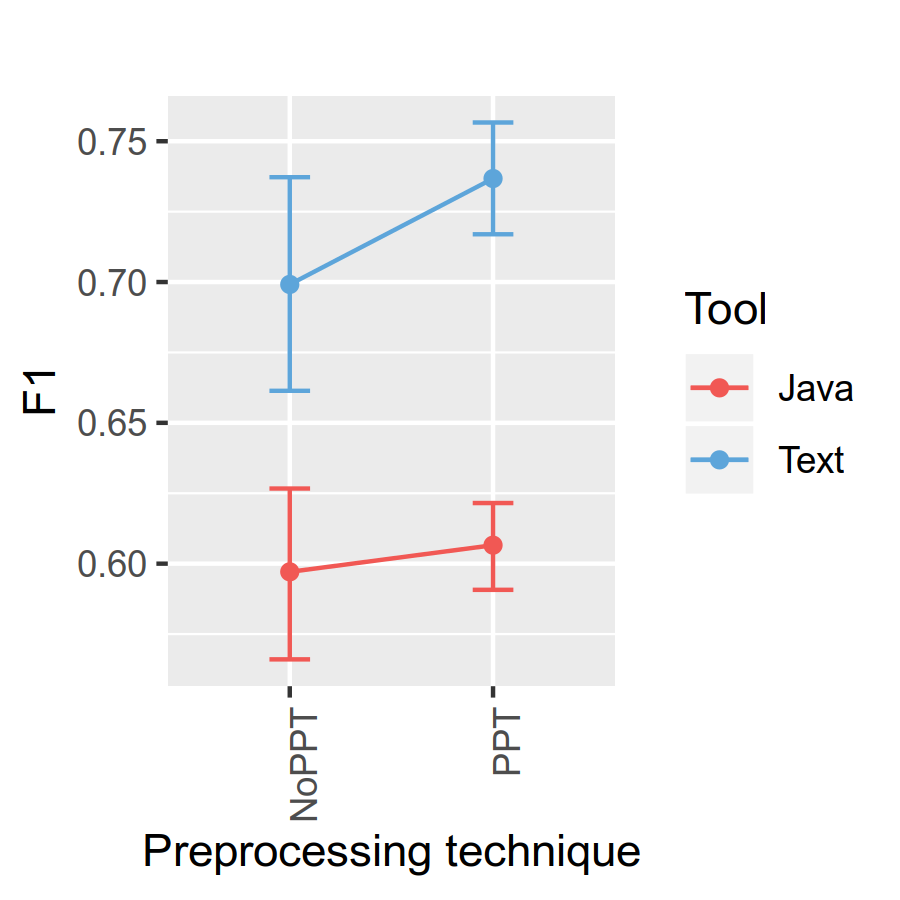
\includegraphics[width=\maxwidth]{figure/Figure-SOCO-INTERACTION-1} 
\subcaption{Interaction  1 }\label{fig:interaction- 1 for SOCO D1 }\endminipage\hfill \minipage{0.32\textwidth} 
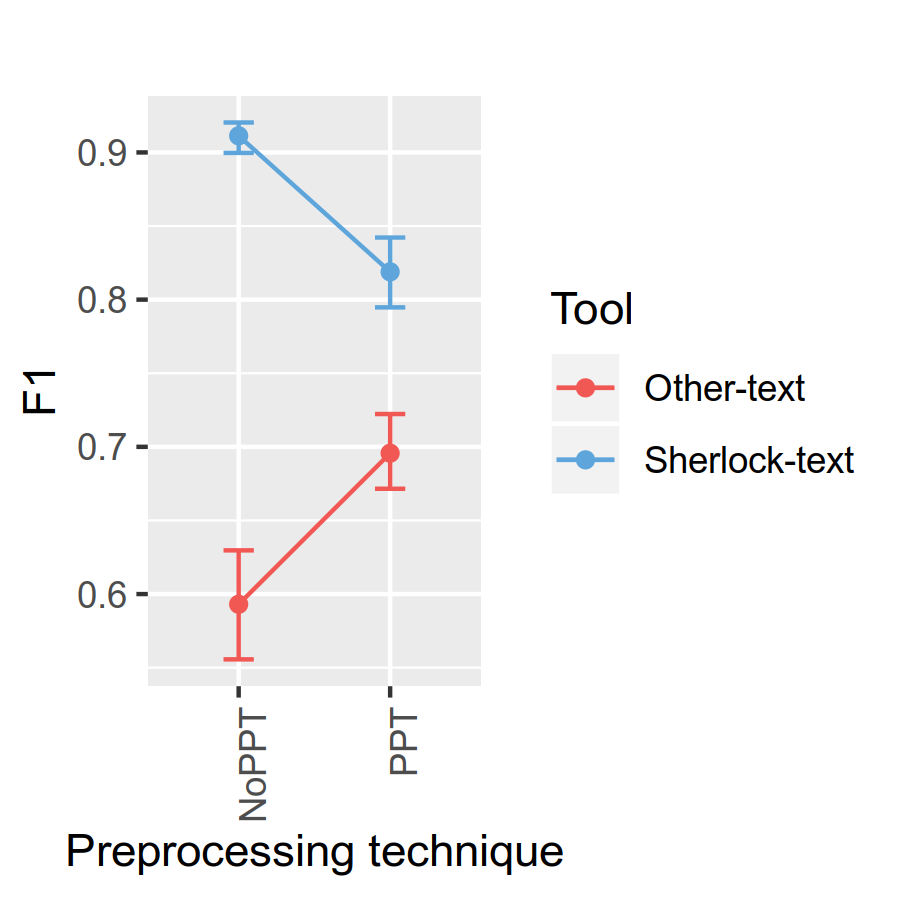
\includegraphics[width=\maxwidth]{figure/Figure-SOCO-INTERACTION-2} 
\subcaption{Interaction  2 }\label{fig:interaction- 2 for SOCO D1 }\endminipage\hfill \minipage{0.32\textwidth} 
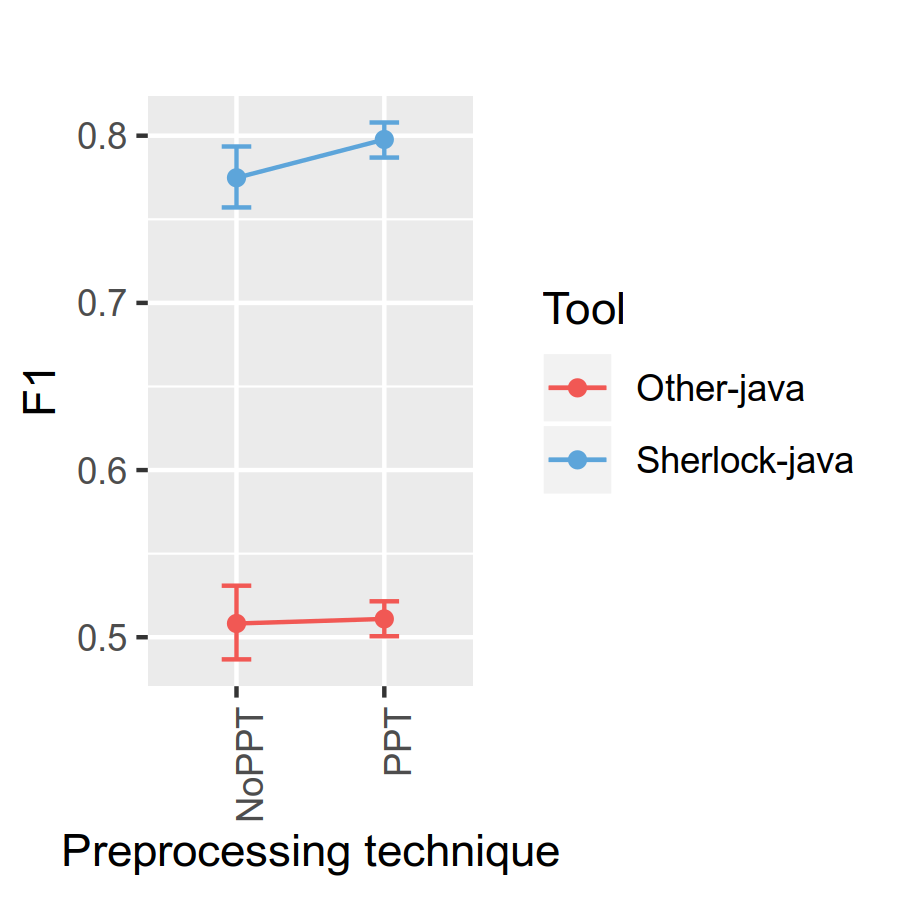
\includegraphics[width=\maxwidth]{figure/Figure-SOCO-INTERACTION-3} 
\subcaption{Interaction  3 }\label{fig:interaction- 3 for SOCO D1 }\endminipage\hfill \minipage{0.32\textwidth} 
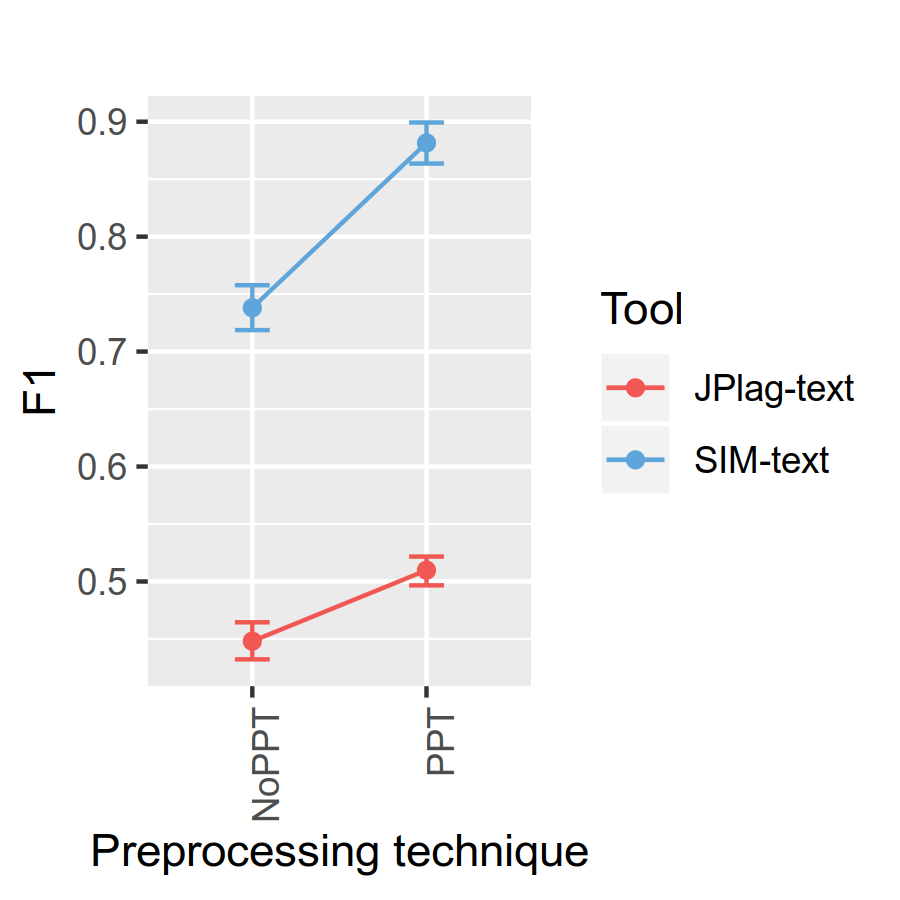
\includegraphics[width=\maxwidth]{figure/Figure-SOCO-INTERACTION-4} 
\subcaption{Interaction  4 }\label{fig:interaction- 4 for SOCO D1 }\endminipage\hfill \minipage{0.32\textwidth} 
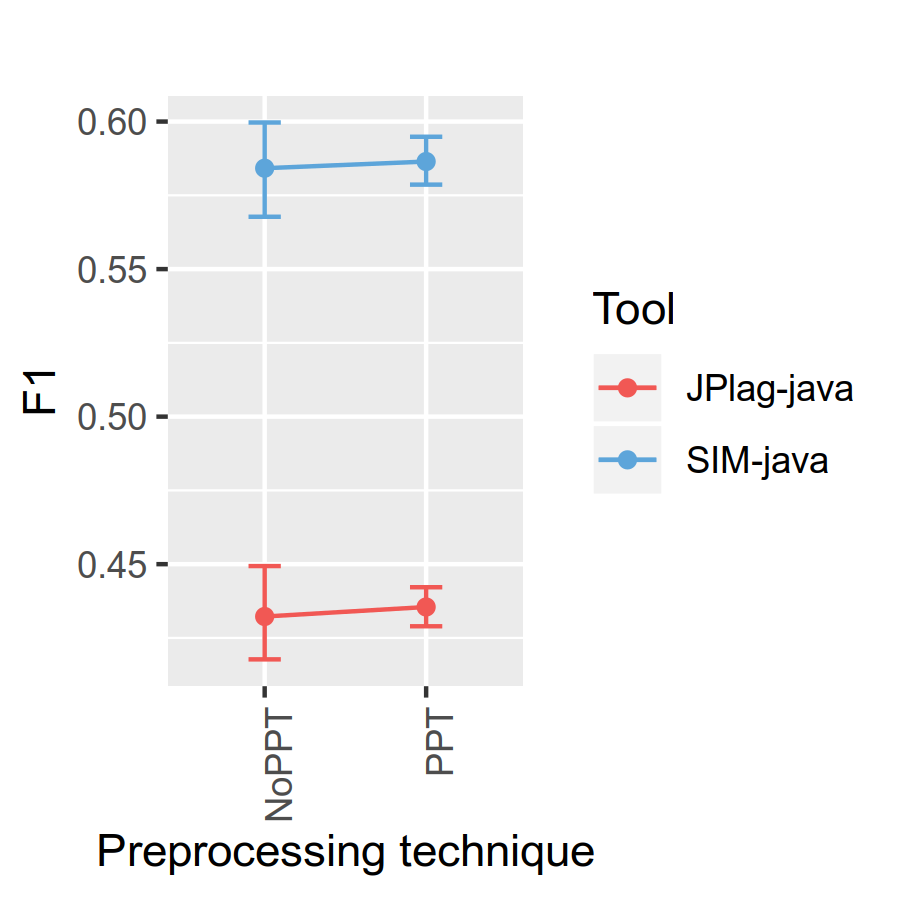
\includegraphics[width=\maxwidth]{figure/Figure-SOCO-INTERACTION-5} 
\subcaption{Interaction  5 }\label{fig:interaction- 5 for SOCO D1 }\endminipage\hfill \minipage{0.32\textwidth} 
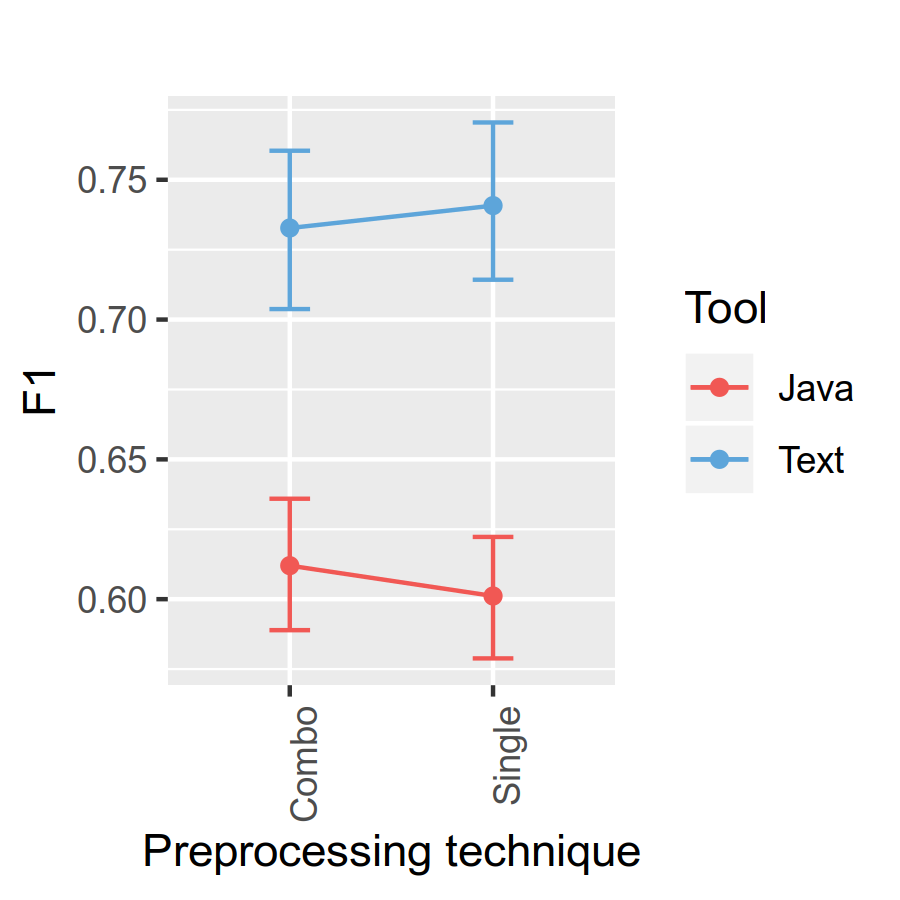
\includegraphics[width=\maxwidth]{figure/Figure-SOCO-INTERACTION-6} 
\subcaption{Interaction  6 }\label{fig:interaction- 6 for SOCO D1 }\endminipage\hfill \minipage{0.32\textwidth} 
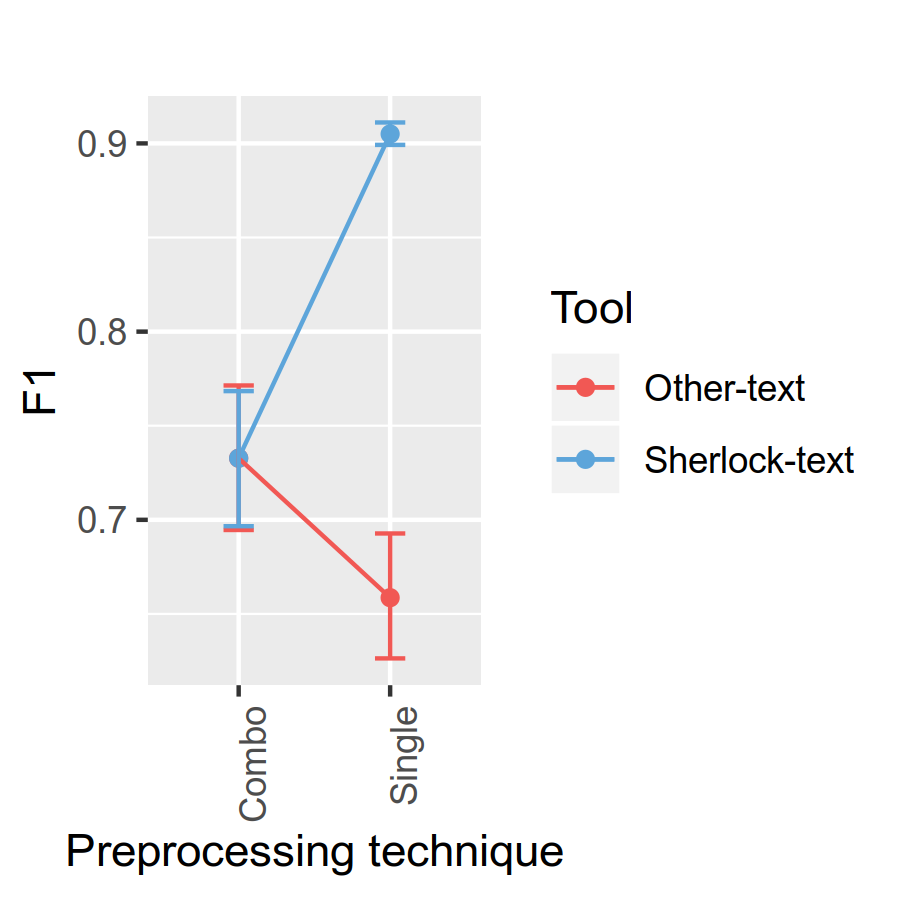
\includegraphics[width=\maxwidth]{figure/Figure-SOCO-INTERACTION-7} 
\subcaption{Interaction  7 }\label{fig:interaction- 7 for SOCO D1 }\endminipage\hfill \minipage{0.32\textwidth} 
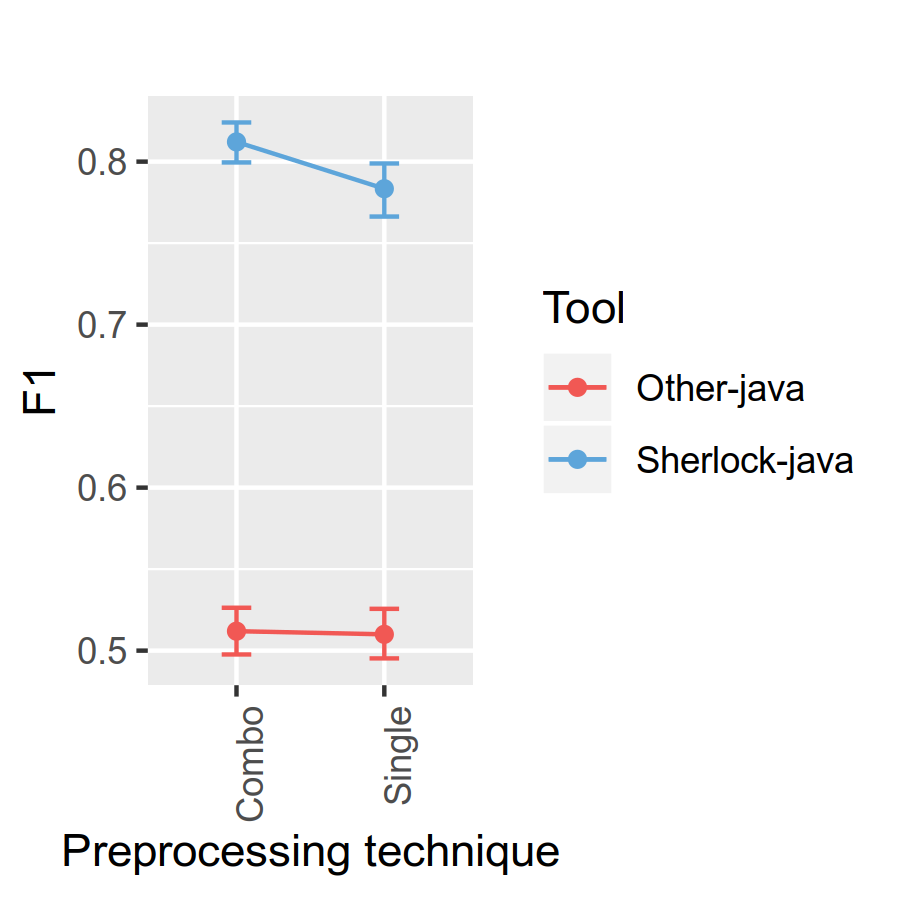
\includegraphics[width=\maxwidth]{figure/Figure-SOCO-INTERACTION-8} 
\subcaption{Interaction  8 }\label{fig:interaction- 8 for SOCO D1 }\endminipage\hfill \minipage{0.32\textwidth} 
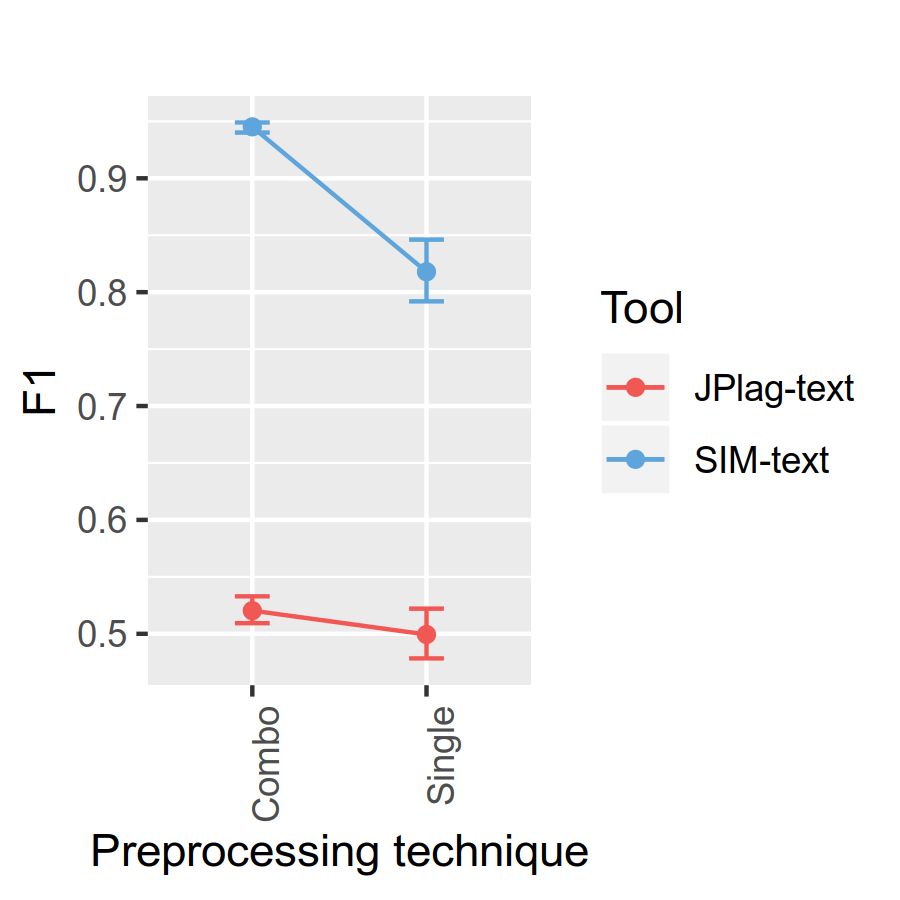
\includegraphics[width=\maxwidth]{figure/Figure-SOCO-INTERACTION-9} 
\subcaption{Interaction  9 }\label{fig:interaction- 9 for SOCO D1 }\endminipage\hfill \caption{Interaction graphs for  SOCO D1  - part 1}\label{fig:interaction SOCO D1 -part1}\end{figure}\begin{figure}[ht]\centering\minipage{0.32\textwidth} 
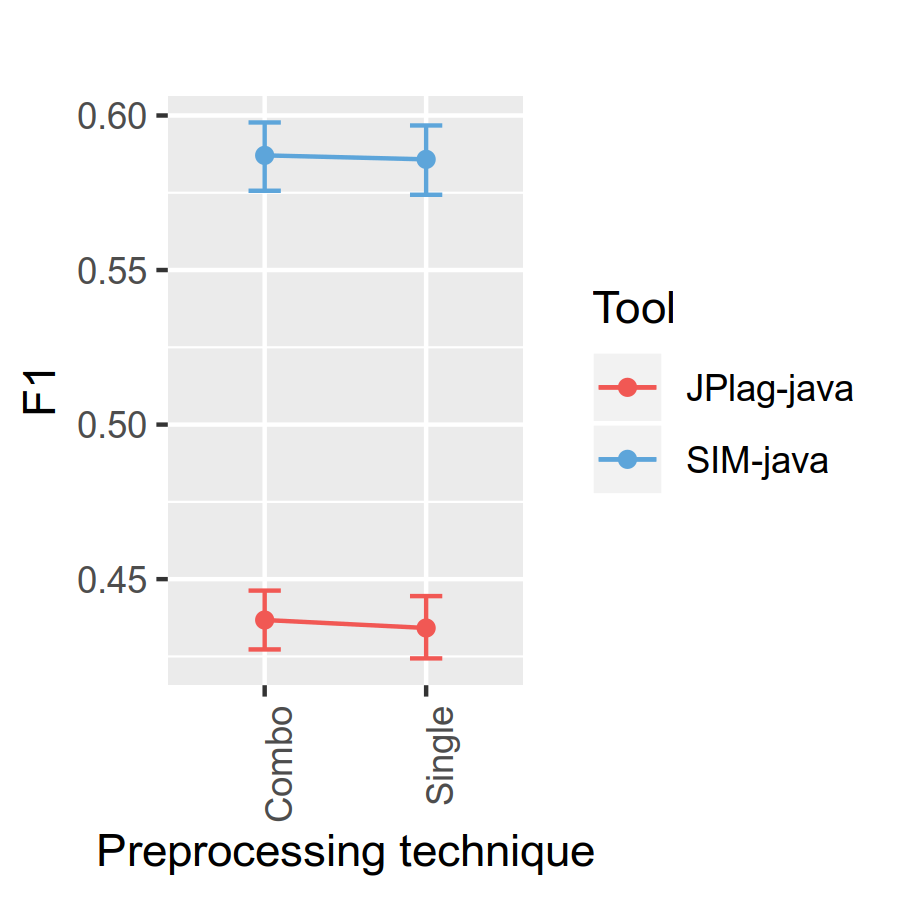
\includegraphics[width=\maxwidth]{figure/Figure-SOCO-INTERACTION-10} 
\subcaption{Interaction  10 }\label{fig:interaction- 10 for SOCO D1 }\endminipage\hfill \minipage{0.32\textwidth} 
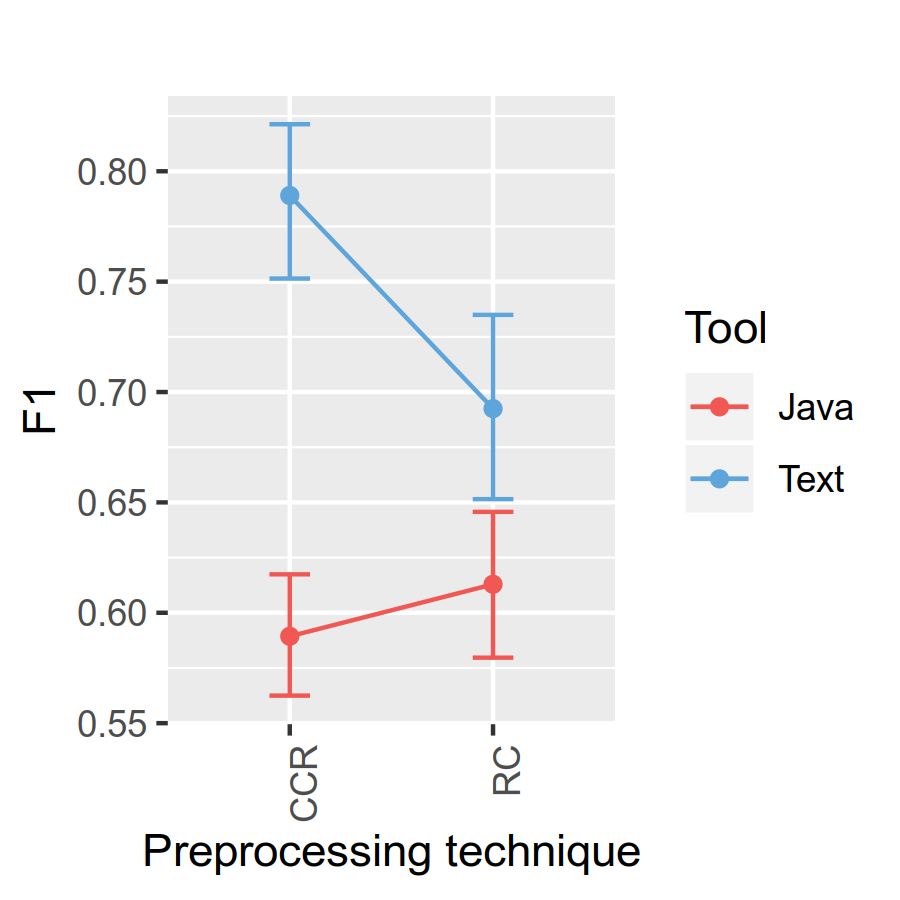
\includegraphics[width=\maxwidth]{figure/Figure-SOCO-INTERACTION-11} 
\subcaption{Interaction  11 }\label{fig:interaction- 11 for SOCO D1 }\endminipage\hfill \minipage{0.32\textwidth} 
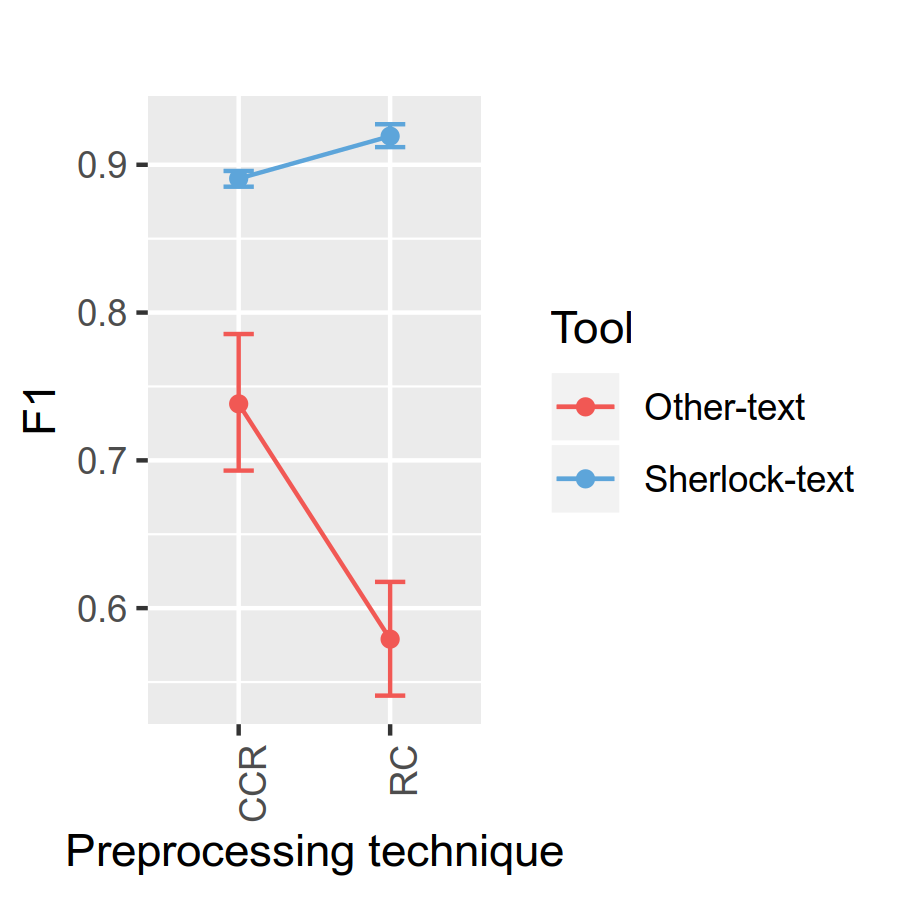
\includegraphics[width=\maxwidth]{figure/Figure-SOCO-INTERACTION-12} 
\subcaption{Interaction  12 }\label{fig:interaction- 12 for SOCO D1 }\endminipage\hfill \minipage{0.32\textwidth} 
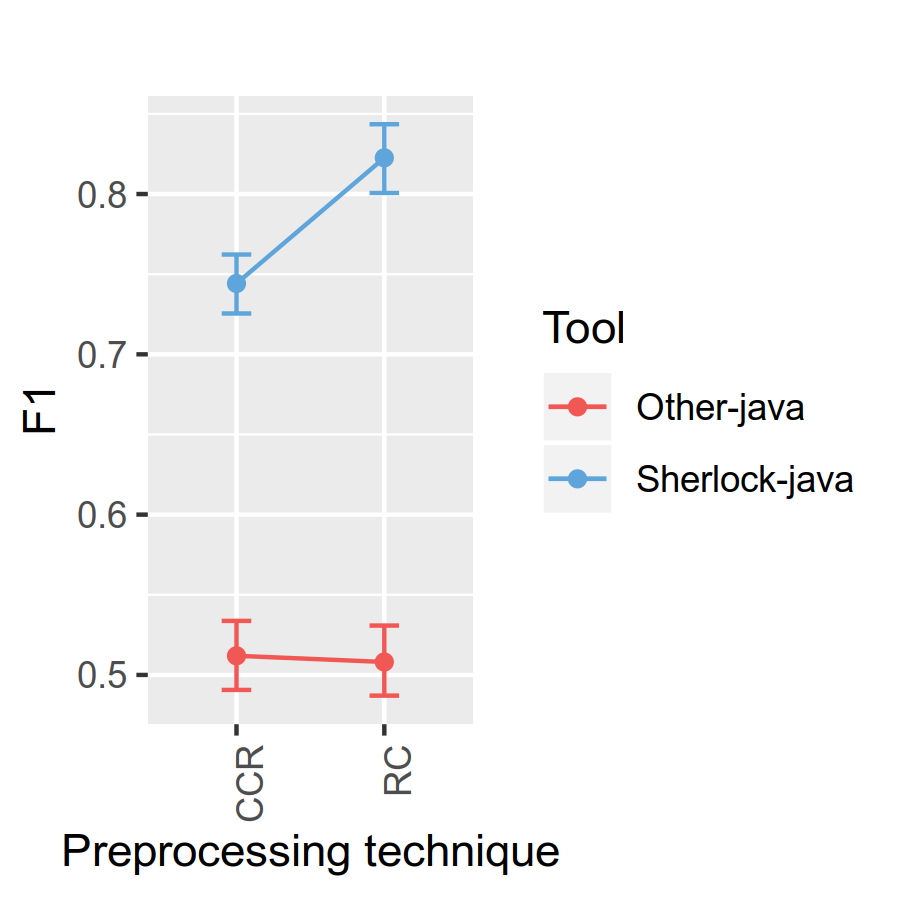
\includegraphics[width=\maxwidth]{figure/Figure-SOCO-INTERACTION-13} 
\subcaption{Interaction  13 }\label{fig:interaction- 13 for SOCO D1 }\endminipage\hfill \minipage{0.32\textwidth} 
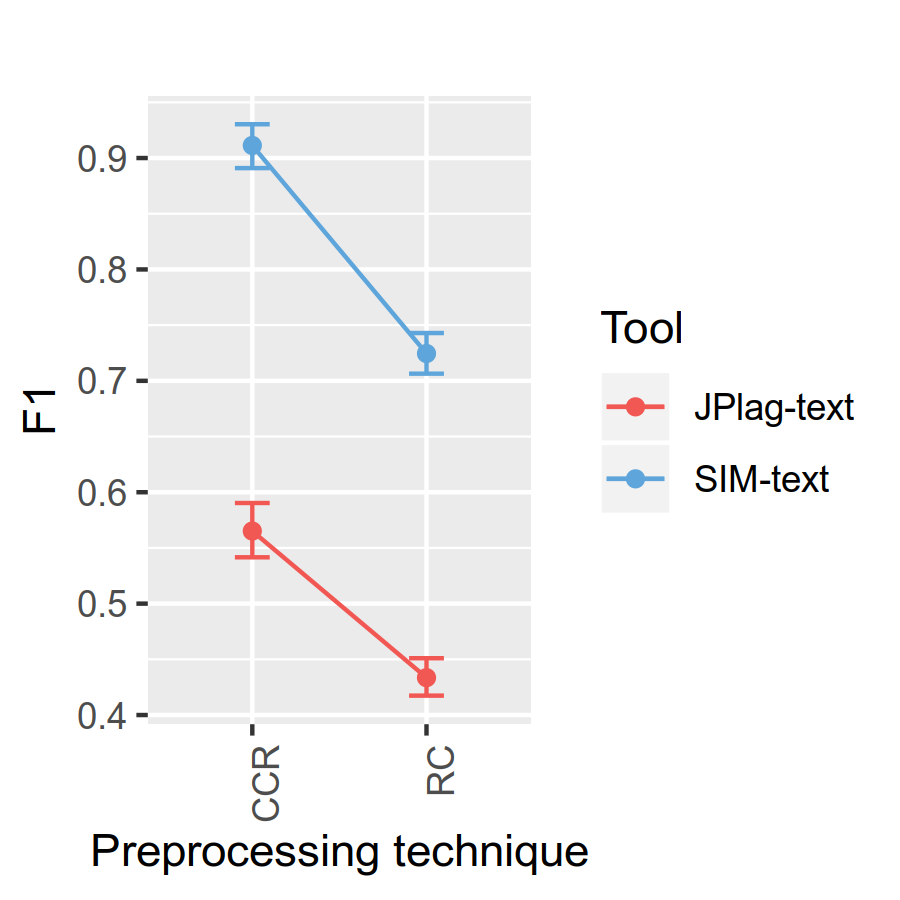
\includegraphics[width=\maxwidth]{figure/Figure-SOCO-INTERACTION-14} 
\subcaption{Interaction  14 }\label{fig:interaction- 14 for SOCO D1 }\endminipage\hfill \minipage{0.32\textwidth} 
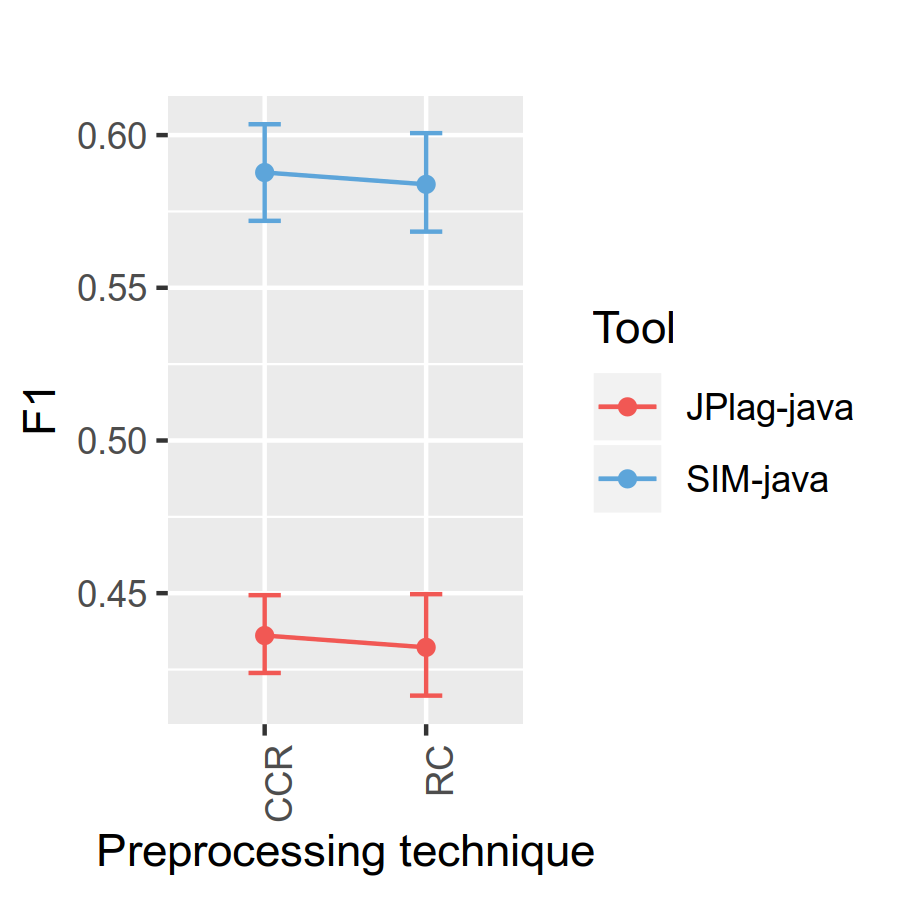
\includegraphics[width=\maxwidth]{figure/Figure-SOCO-INTERACTION-15} 
\subcaption{Interaction  15 }\label{fig:interaction- 15 for SOCO D1 }\endminipage\hfill \minipage{0.32\textwidth} 
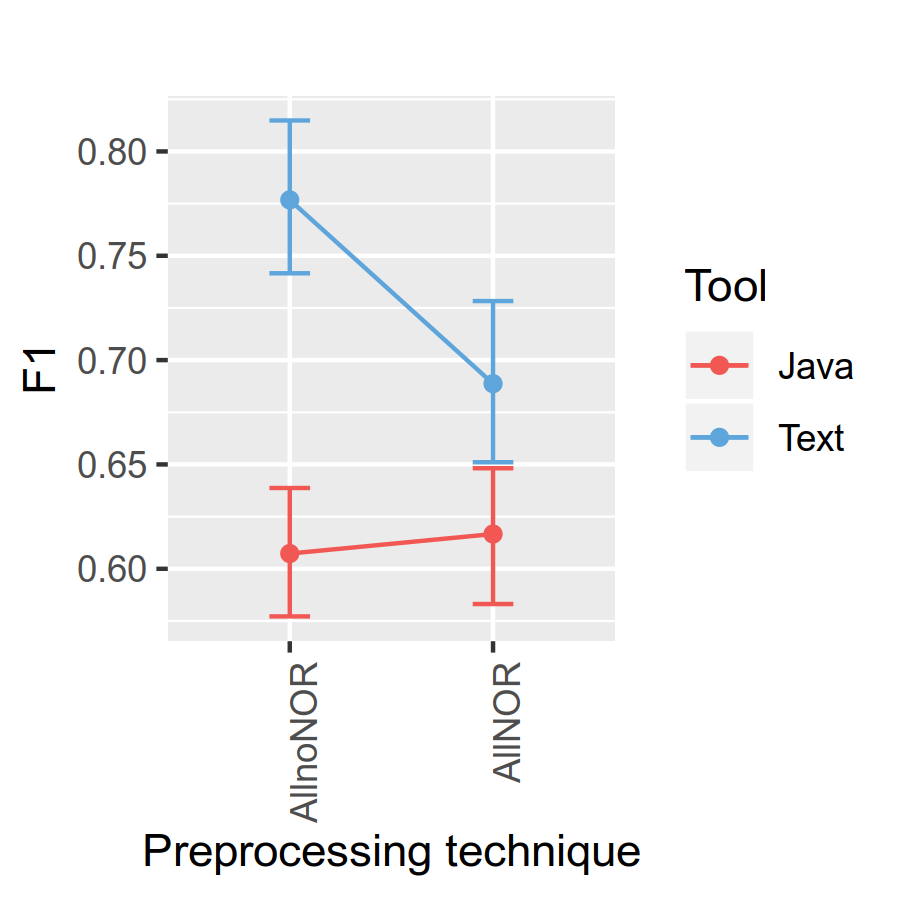
\includegraphics[width=\maxwidth]{figure/Figure-SOCO-INTERACTION-16} 
\subcaption{Interaction  16 }\label{fig:interaction- 16 for SOCO D1 }\endminipage\hfill \minipage{0.32\textwidth} 
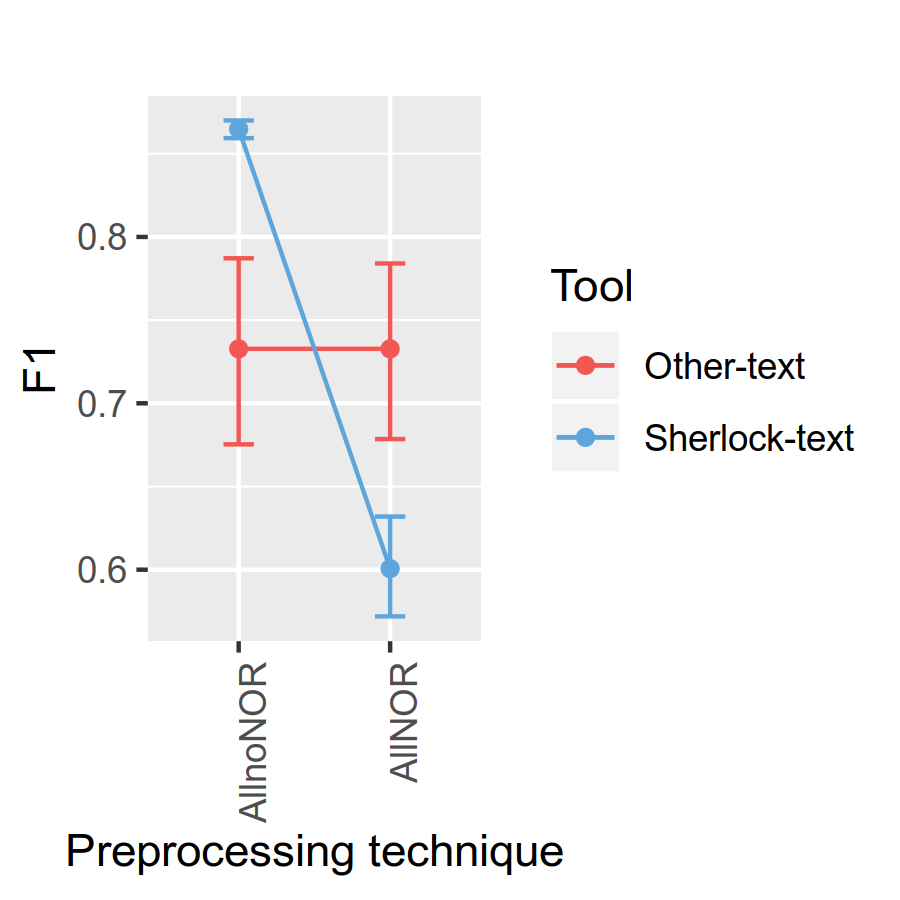
\includegraphics[width=\maxwidth]{figure/Figure-SOCO-INTERACTION-17} 
\subcaption{Interaction  17 }\label{fig:interaction- 17 for SOCO D1 }\endminipage\hfill \minipage{0.32\textwidth} 
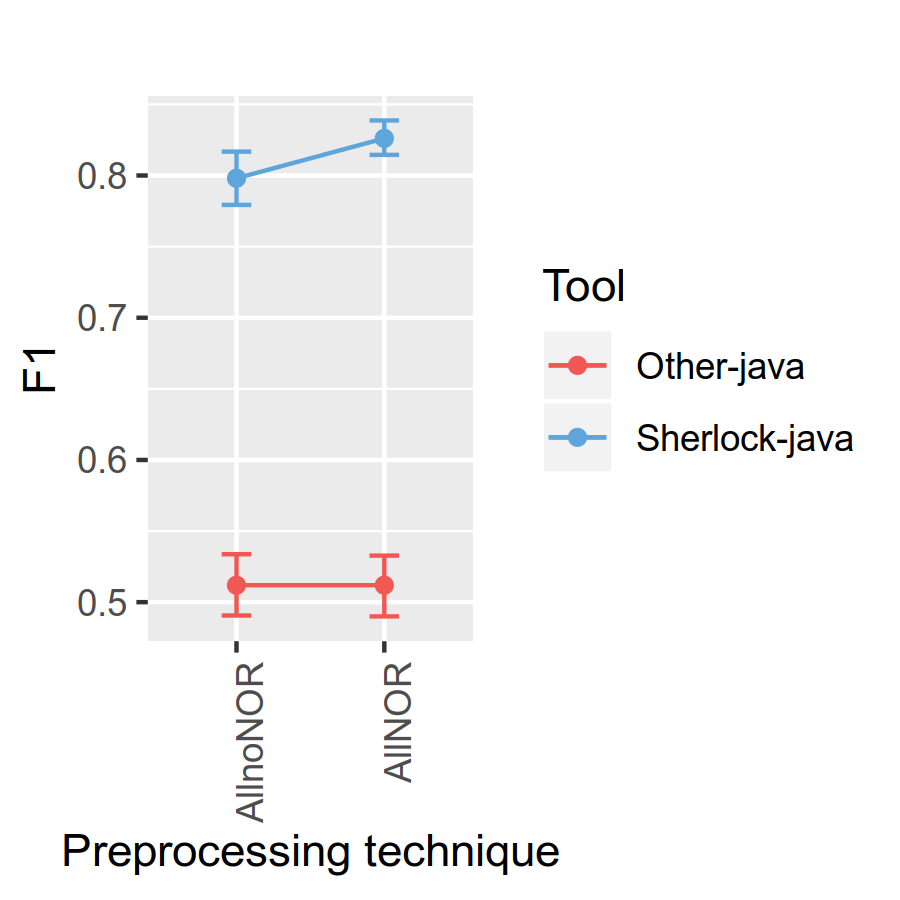
\includegraphics[width=\maxwidth]{figure/Figure-SOCO-INTERACTION-18} 
\subcaption{Interaction  18 }\label{fig:interaction- 18 for SOCO D1 }\endminipage\hfill \minipage{0.32\textwidth} 
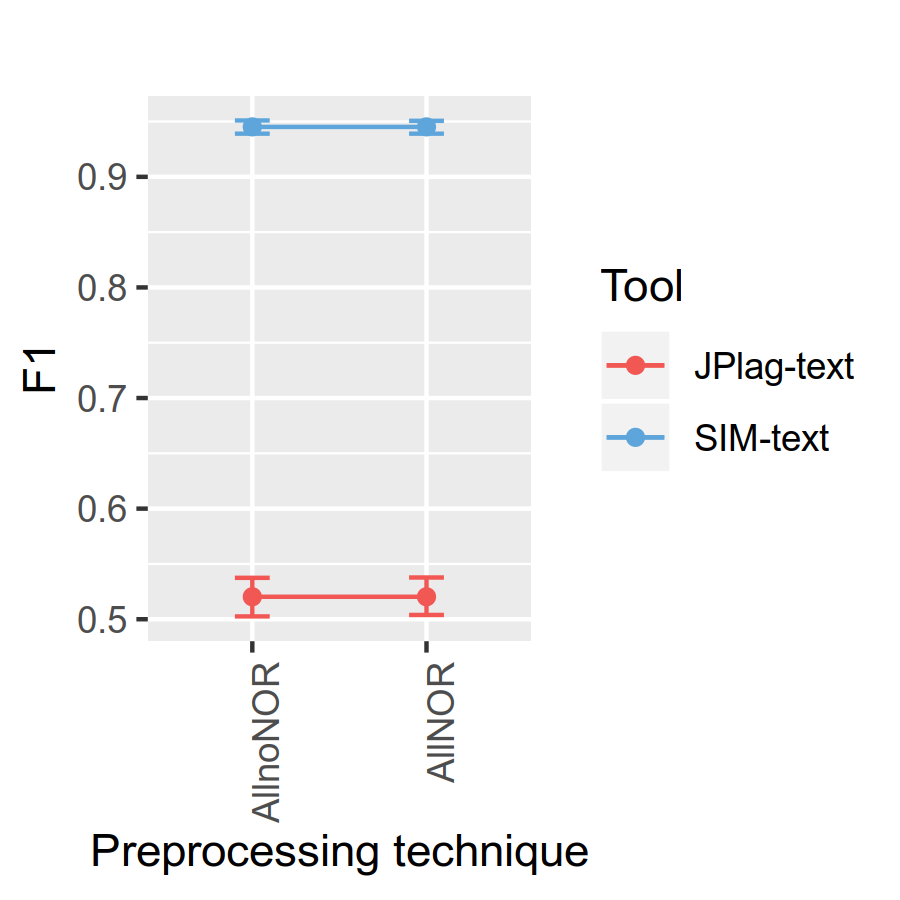
\includegraphics[width=\maxwidth]{figure/Figure-SOCO-INTERACTION-19} 
\subcaption{Interaction  19 }\label{fig:interaction- 19 for SOCO D1 }\endminipage\hfill \minipage{0.32\textwidth} 
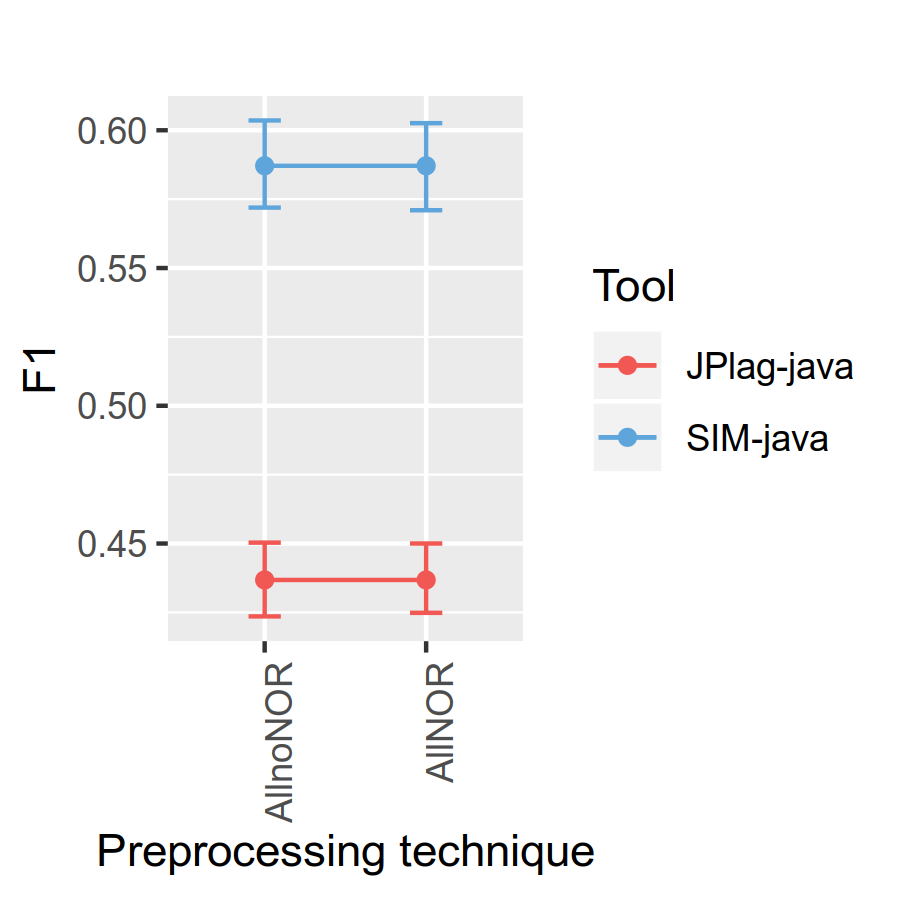
\includegraphics[width=\maxwidth]{figure/Figure-SOCO-INTERACTION-20} 
\subcaption{Interaction  20 }\label{fig:interaction- 20 for SOCO D1 }\endminipage\hfill \caption{Interaction graphs for  SOCO D1  - part 2}\label{fig:interaction SOCO D1 -part2}\end{figure}
\end{appendices}
    \printbibliography[heading=bibintoc, notcategory=fullcited]
  
  \backmatter
  \pdfbookmark[0]{Curiculum Vite}{cv}
\chapter*{Curiculum Vite}

\lipsum[1-4]

\ldots

\begin{center}
	\Large Bibliography
\end{center}


\mybibexclude{novak2019}

\pdfbookmark[1]{Bibliography}{myBibliography}
\begin{easylist}[enumerate]
& \fullcite{novak2019}
& \fullcite{hebb1985social}
\end{easylist}

\thispagestyle{empty}


    
\end{document}
